\section{Experimental Results}
\label{sec:results}

\subsection{RQ1: SUIT Smells Identification}
\label{sec:results-smells-collection}

Figure~\ref{fig:smell-sources} shows the number of test smells that were found in academic and grey literature. We show both the 35 initial \gls{suit} smells extracted from the literature and the subset of 16 \gls{suit} smells for which we could extract a metric in the test code.

In the figure, a \gls{suit} smell is considered as covered by academia if at least one of the smells grouped in the generalization step (Section~\ref{sec:experience-design-smells-collection}) is covered by a peer-reviewed article. Interestingly, all smells covered by academic literature appear in grey literature as well. The figure shows that while there exists an interest from practitioners with 35 unique smells discussed, the number of smells discussed in peer-reviewed literature remains rather limited with only 10 \gls{suit} smells identified. Furthermore, smells identified from the literature could generate a metric in six out of ten cases. The ones for which no metric could be derived are \emph{Inconsistent Wording} \cite{Hauptmann2013}, \emph{Unsuitable Naming} \cite{Chen2012}, \emph{Inconsistent Hierarchy} \cite{Hauptmann2013} and \emph{Data Creep} \cite{Alegroth2016b}. While \cite{Hauptmann2013} propose metrics for the smells they introduce, during our evaluation we observed a high rate of false positive for \emph{Inconsistent Wording} and \emph{Inconsistent Hierarchy} thus we excluded them for the final list. \cite{Chen2012} and \cite{Alegroth2016b} on the other hand do not propose a metric to automatically extract symptoms for the smells they present. 

To conclude this analysis of Figure~\ref{fig:smell-sources}, we see that there exists a gap between the grey literature and the academic literature. We believe that more work need to be conducted to better understand and automatically detect and refactor \gls{suit} smells in the academia. The present work is an attempt to fill this gap with the introduction of 25 new \gls{suit} smells not previously studied in academia.

Figure~\ref{fig:smell-issues} presents the effects associated to each \gls{suit} smell. Note that a smell can lead to issues from different categories. Thus, the total number of issues is greater than the number of smells. From the figure, we observe that although readability issues appear the most often with 18 instances, maintenance issues with 12 instances and execution issues with 14 instances do not fall far behind. Furthermore, to our surprise, \gls{suit} smells affecting readability are the ones for which the highest number of metrics could be computed. One reason explaining this phenomenon is that in the case of execution issues, information about the \gls{sut} and its execution are required. The same observation can be made for maintenance where the danger is coming from a divergence of the test from the \gls{sut} as it is the case for instance with the \emph{Lifeless} smell \cite{Buwalda2015, Renaudin2016, Buwalda2019} where the test is not following the same lifecycle as the application. Thus, in both cases, the extraction of the symptoms requires information about the structure and lifecycle of the \gls{sut}.

\begin{figure}
\centering
\subfloat[Source]{ 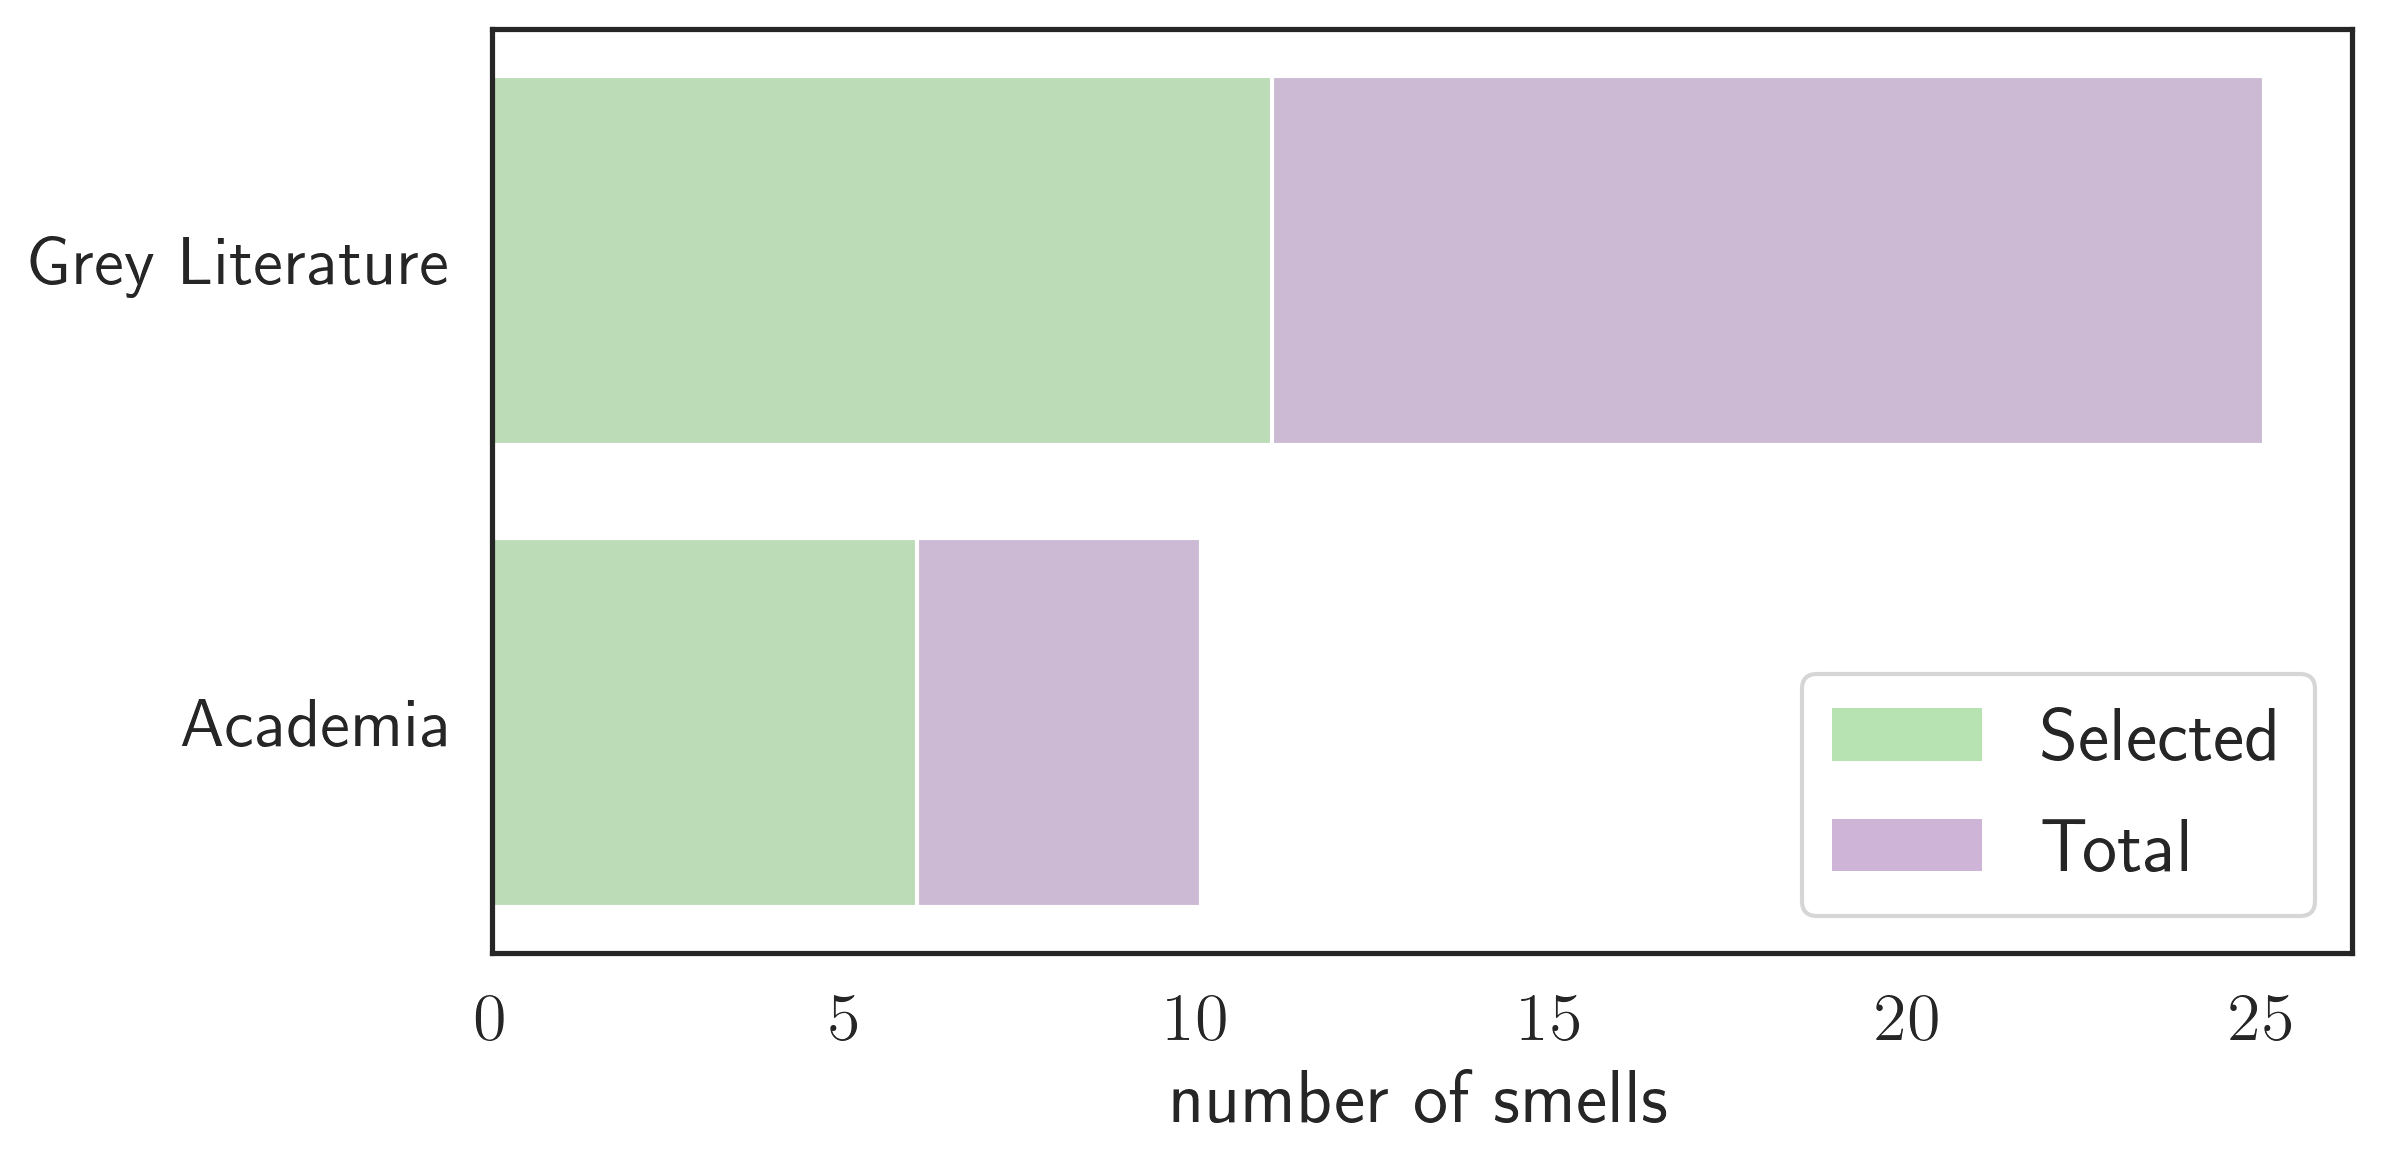
\includegraphics[width=0.45\linewidth]{figures/smells/source-distribution-acceptance.png}\label{fig:smell-sources}}
\subfloat[Issues]{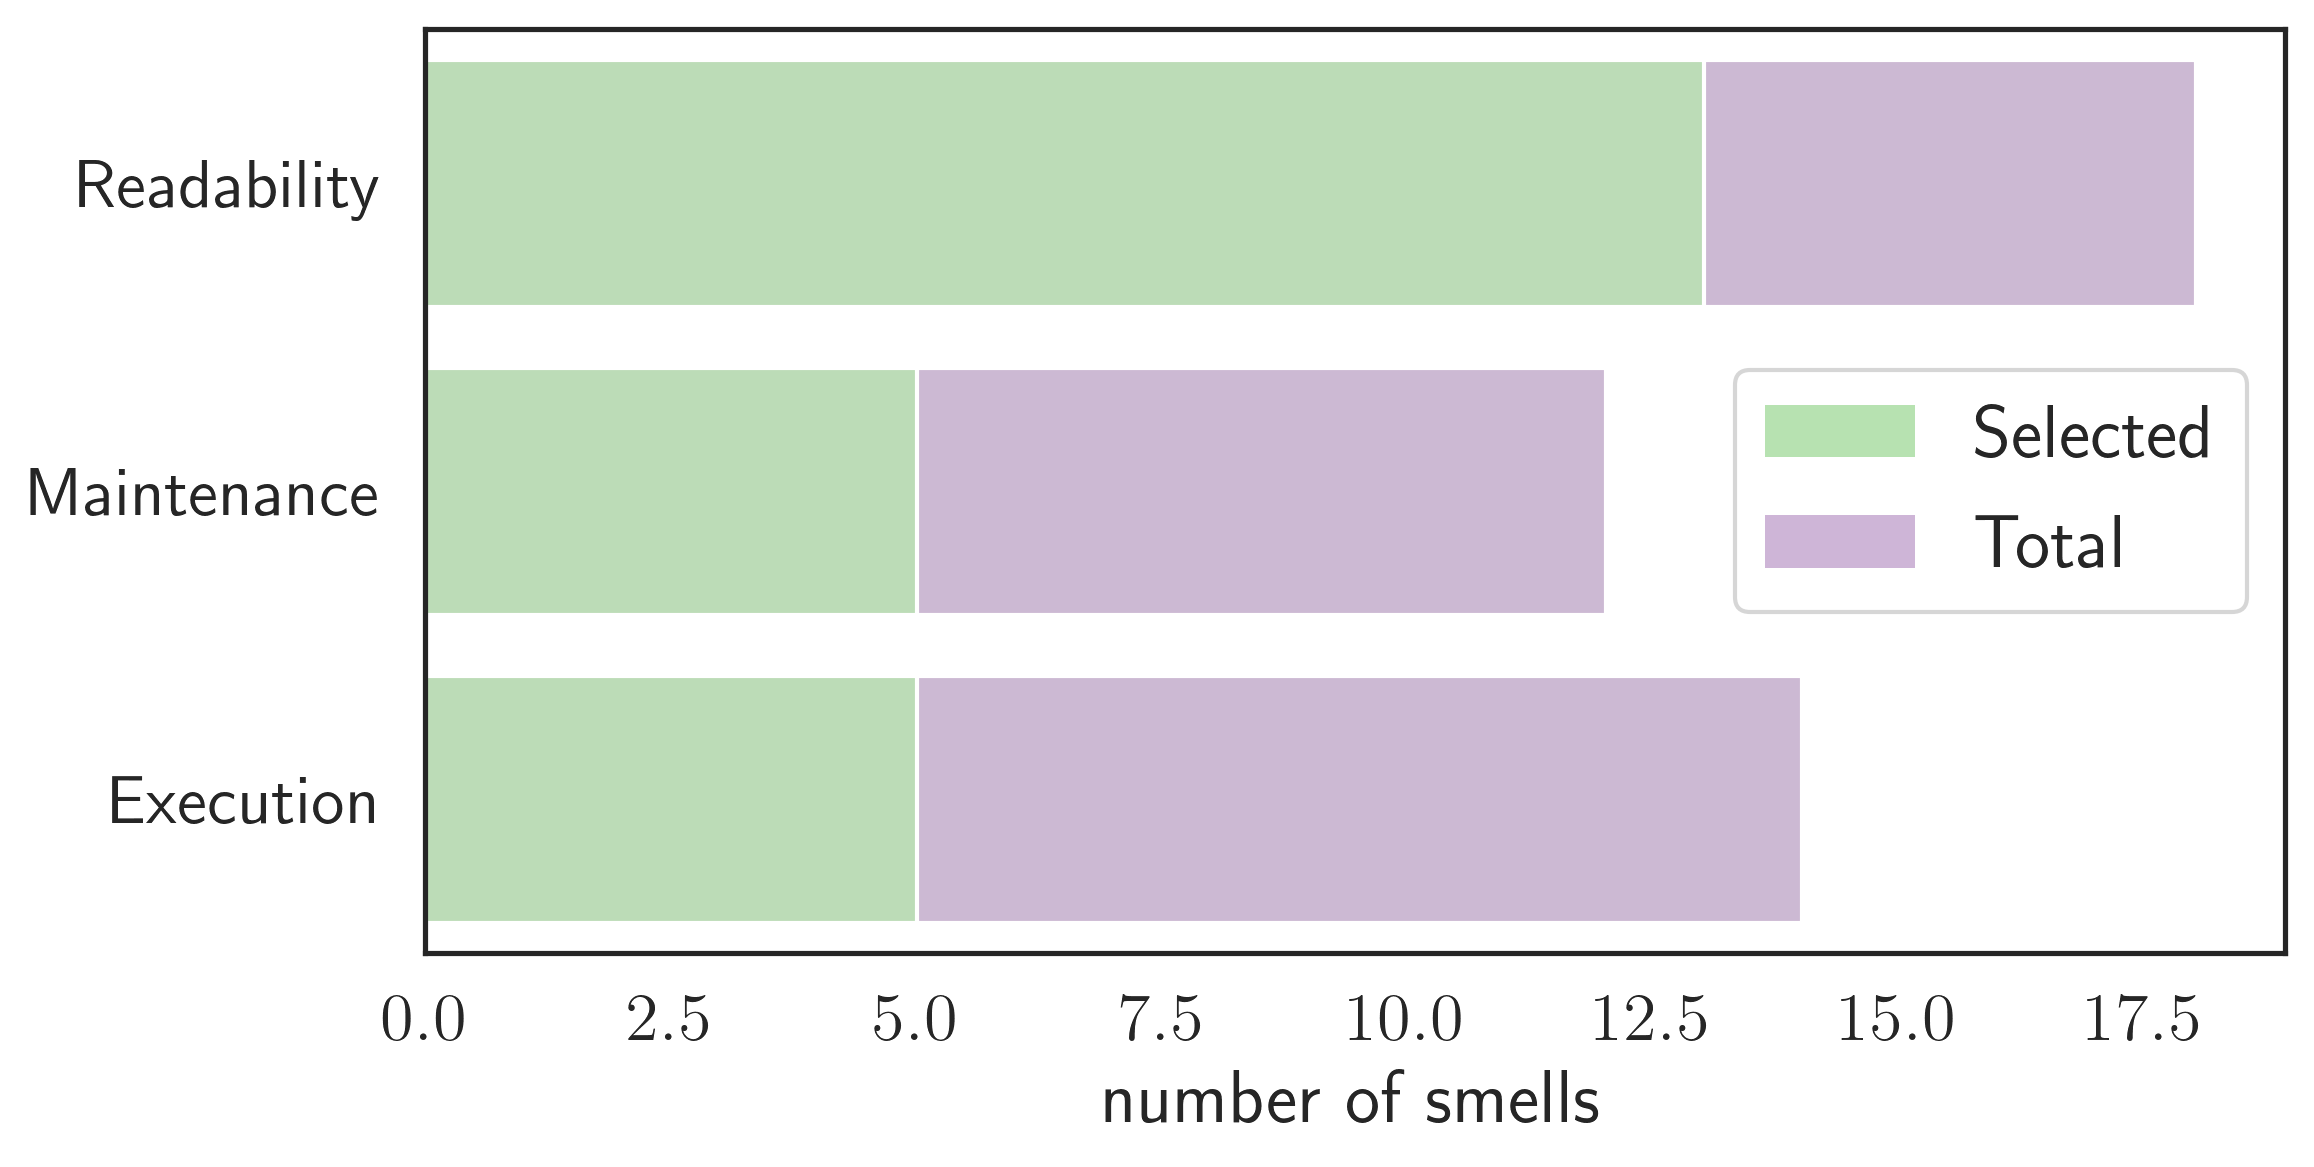
\includegraphics[width=0.45\linewidth]{figures/smells/issue-distribution-acceptance.png}\label{fig:smell-issues}}
\caption{Properties of the identified \gls{suit} smells. Figure~\ref{fig:smell-sources} displays the number of smells found in the academic and in the grey literature. Figure~\ref{fig:smell-issues} displays the number of smells exhibiting a specific issue. Note that a smell can lead to one type of issue, hence the total is greater than the total number of \gls{suit} smells.}  
\label{fig:smells}
\end{figure}

\subsection{SUIT Smells Catalog}
\label{sec:results-smells-catalog}

The process described in section~\ref{sec:experience-design-smells-collection} leads to a final list of 35 \gls{suit} smells presented in Table~\ref{tab:smell-catalog}. Out of those 35 \gls{suit} smells, we conduct a deeper analysis on 16 of them, the ones for which a metric can be automatically derived by observing Robot Framework test code.

\begin{table}
\centering

\caption{Catalog of SUIT Smells and their origin. Smell in bold are associated with a metric and a complete description is presented in Section~\ref{sec:results-smells-catalog}.}
\label{tab:smell-catalog}.

\begin{tabular}{>{\raggedright}p{1.5in}>{\raggedright}p{4in}}

\toprule
\scriptsize{\textbf{Name}} & \scriptsize{\textbf{Sources}}\tabularnewline
\toprule

\scriptsize{\textbf{Army of Clones}} & \scriptsize{\cite{Chen2012, Hauptmann2013, Hauptmann2015, Jones2019}} \tabularnewline 


\scriptsize{Complicated Setup Scenarios} & \scriptsize{\cite{Scott2015}} \tabularnewline 

\scriptsize{\textbf{Conditional Assertions}} & \scriptsize{\cite{Gawinecki2016}} \tabularnewline 

\scriptsize{Conspiracy Of Silence} & \scriptsize{\cite{Gawinecki2016, Sheth2020}} \tabularnewline 

\scriptsize{Data Creep} & \scriptsize{\cite{Alegroth2016b, Siminiuc2019, Shay2019}} \tabularnewline 

\scriptsize{Dependencies between tests} & \scriptsize{\cite{Klarck2014, Advolodkin2018, Cripsin2018, Bushnev2019, Goldberg2019}} \tabularnewline 

\scriptsize{Directly Executing UI Scripts} & \scriptsize{\cite{Scott2015}} \tabularnewline 

\scriptsize{Duplicate Check} & \scriptsize{\cite{Buwalda2019}} \tabularnewline 

\scriptsize{Eager Test} &  \scriptsize{\cite{England2016, Renaudin2016, Cripsin2018, Sciamanna2019, Temov2020}} \tabularnewline 

\scriptsize{\textbf{Hardcoded Environment}} & \scriptsize{\cite{Gawinecki2016, Sheth2020}} \tabularnewline 

\scriptsize{\textbf{Hiding Test Data}} & \scriptsize{\cite{Jain2007}} \tabularnewline 

\scriptsize{Implementation Dependent}  & \scriptsize{\cite{Jain2007, Kapelonis2018, Goldberg2019}} \tabularnewline 

\scriptsize{Inconsistent Hierarchy} & \scriptsize{\cite{Clayton2014, Gawinecki2016, Buwalda2019}} \tabularnewline 

\scriptsize{Inconsistent Wording} & \scriptsize{\cite{Hauptmann2013}} \tabularnewline 

\scriptsize{\textbf{Lack of Encapsulation}} & \scriptsize{\cite{Chen2012, Evangelisti2012, Klarck2014, Buwalda2015, England2016, Renaudin2016, Knight2017a, Goldberg2019, Jones2019, Shay2019}} \tabularnewline 

\scriptsize{Lack Of Early Feedback} & \scriptsize{\cite{Dharmender2017}} \tabularnewline 

\scriptsize{Lifeless} & \scriptsize{\cite{Buwalda2015, Renaudin2016, Buwalda2019}} \tabularnewline 

\scriptsize{\textbf{Long Test Steps}} & \scriptsize{\cite{Chen2012, Hauptmann2013, Buwalda2019}} \tabularnewline

\scriptsize{\textbf{Middle Man}} & \scriptsize{\cite{Chen2012}} \tabularnewline 

\scriptsize{\textbf{Missing Assertion}} & \scriptsize{\cite{Klarck2014}} \tabularnewline 

\scriptsize{\textbf{Narcissistic}} & \scriptsize{\cite{England2016, Knight2017b}.} \tabularnewline

\scriptsize{\textbf{Noisy Logging}} & \scriptsize{\cite{Jain2007}.} \tabularnewline

\scriptsize{\textbf{Obscure Test}} & \scriptsize{\cite{Hauptmann2013, Gawinecki2016, Siminiuc2019}.} \tabularnewline

\scriptsize{\textbf{On the Fly}} & \scriptsize{\cite{Archer2010}} \tabularnewline 

\scriptsize{\textbf{Over-Checking}} & \scriptsize{\cite{Buwalda2015, Renaudin2016}} \tabularnewline

\scriptsize{Pointless Descriptions} & \scriptsize{\cite{England2016}} \tabularnewline 

\scriptsize{\textbf{Sensitive Locators}} & \scriptsize{\cite{Scott2015, Jones2019, Battat2020, Sheth2020}} \tabularnewline

\scriptsize{\textbf{Sneaky Checking}} & \scriptsize{\cite{Kirkbride2014, Buwalda2015, Renaudin2016}} \tabularnewline

\scriptsize{\textbf{Stinky Synchronization}} & \scriptsize{\cite{Gawinecki2016, Renaudin2016, Bushnev2019, Jones2019, Sheth2020}} \tabularnewline 

\scriptsize{Test Data Loss} & \scriptsize{\cite{Siminiuc2019}} \tabularnewline

\scriptsize{Testing Data Not Code} & \scriptsize{\cite{Dharmender2017}} \tabularnewline 

\scriptsize{Unnecessary Navigation} & \scriptsize{\cite{Archer2010}} \tabularnewline 

\scriptsize{Unrealistic Data} & \scriptsize{\cite{Goldberg2019}} \tabularnewline 

\scriptsize{Unsecured Test Data} & \scriptsize{\cite{Morlion2019}} \tabularnewline

\scriptsize{Unsuitable Naming} & \scriptsize{\cite{Chen2012, Goldberg2019, Shay2019, Sheth2020}} \tabularnewline

\bottomrule
\end{tabular}

\end{table}

Building on the tree model introduced in Section~\ref{sec:tree-representation-KDT} we represent each test $t$ as a rooted, ordered, directed, acyclic graph. The nodes, $N_t$, of the tree represent the set of calls to \emph{Keywords}, $C_t$, and the set of of arguments $A$ passed to the calls. A call, $c_t$, can be associated to a type namely: USER, INTERACTION, ASSERTION, CONTROLFLOW, GETTER, LOGGING and SYNC. For example, the set of calls in a test performing an assertion is noted $C_{t, assertion}$. Finally, the definition of the \emph{User Kyeword} called by a test $t$ is noted $K_t$. Following this notation, we formally describe each smell with respect to its symptoms, its impact, and the metrics chosen to measure the prevalence of the symptoms following the protocol presented in Section~\ref{sec:smell-detection}. Finally, we present the refactoring actions removing the symptoms from the test code base.

\subsubsection{Army of Clones (AoC)}

\begin{itemize}
    \item \textbf{Description:} Different tests perform and implement similar actions, leading to duplicated pieces of test code.
    
    \item \textbf{Impact on Readability:} Test sequences which are similar but not identical are not easy to distinguish. It is not easy to grasp the intention of the test in comparison with its clone.
    
    \item \textbf{Impact on Maintenance:} The effort to maintain duplicated parts of tests increases. Furthermore, it is difficult to determine where maintenance has to be performed.
    
    \item \textbf{Detection Method:} Code duplication can be observed at different levels. Here, for the body of a \emph{User Keyword}, we detect if there exists a clone of type 1 (code duplication at the token level) or type 2 (code duplication at syntax level allowing for minor syntactic changes such as variables name) in the test suite. Thus, we express the count metric, $S_{AoC}(t)$, as the number of calls to \emph{User Keywords} that have a clone and the density metric, $D_{AoC}(t)$, as the number of calls to \emph{User Keywords} that have a clone over the total number of unique \emph{User Keywords} called by the test. More formally:

    \begin{equation*}
        S_{AoC}(t) = \abs{K_t \cap K_{clone}} 
    \end{equation*}
    
    \begin{equation*}
        D_{AoC}(t) = \frac{\abs{K_t \cap K_{clone}}}{\abs{K_{t}}}
    \end{equation*}
    
    where $K_{t}$ is the set of unique \emph{User Keywords} called by test $t$ and $K_{clone}$ is the set of unique \emph{User Keywords} that have at least one clone in the test suite.
    
    \item \textbf{Refactoring Actions:} The symptom is considered refactored if the \emph{User Keyword} that is called by a test  and have at least one clone in the test suite, $k_{t, clone}$, is removed. Thus, we propose the refactoring pattern, $R_{AoC}(k)$, as follow:

    \begin{equation*}
        R_{AoC}(k) = k_{t, clone} \xrightarrow{action} \emptyset
    \end{equation*}
\end{itemize}

\subsubsection{Conditional Assertions (CA)}

\begin{itemize}
    \item \textbf{Description:} The test verifies different properties depending on the environment when the environment state may change from one execution to the next.
    
    \item \textbf{Impact on Readability:} With more complex logic in the assertions, it becomes harder to capture their meaning.
    
    \item \textbf{Impact on Execution:} More complex code might introduce bugs in the test code.
    
    \item \textbf{Detection Method:} We consider assertions nodes, $C_{assertion}$, to be symptomatic if they have a parent node which is a conditional node and have no sibling nodes in the call graph, $C_{condition}$. Thus, we express the count metric, $S_{CA}(t)$, as the number of conditional assertion calls and the density metric, $D_{CA}(t)$, as the number of conditional assertion calls over the total number of assertion calls.

    \begin{equation*}
        S_{CA}(t) = \abs{C_{t} \cap C_{assertion} \cap C_{condition}}
    \end{equation*}
    
    \begin{equation*}
        D_{CA}(t) = \frac{\abs{C_{t} \cap C_{assertion} \cap C_{condition}}}{\abs{C_{t} \cap C_{assertion}}}
    \end{equation*}
    
    where $\abs{C_{t} \cap C_{assertion}}$ is the size of the set of calls to \emph{Library Keyword} annotated as ``assertion'' for a test $t$ and $\abs{C_{t} \cap C_{assertion} \cap C_{condition}}$  is the size of the set of calls to \emph{Library Keyword} annotated as ``assertion'' for which the caller is a conditional node that has only one child (logging nodes excluded).
    
    \item \textbf{Refactoring Action:} The symptom is considered refactored if the conditional assertion node is removed from the call graph. Thus, we accept the following refactoring pattern, $R_{CA}(c)$, as removing a symptom in a node $c$:

    \begin{equation*}
        R_{CA}(c) =  c_{t, assertion, condition} \xrightarrow{action} c_{t, assertion}
    \end{equation*}
    
    The assertion $c_{t, assertion}$ replaces its former parent node $c_{t, assertion, condition}$. Note that removing a parent of $c_{t, assertion, condition}$ or adding a sibling to the child assertion node are not considered as fixing the symptom.
\end{itemize}

\subsubsection{Hardcoded Environment (HE)}

\begin{itemize}
    \item \textbf{Description:} The test contains hardcoded references to the environment when the same requirement must be run against different test environments instead of having an environment-agnostic test.
    
    \item \textbf{Impact on Maintenance:} Updating the configuration requires modifying multiple locations in different tests.
    
    \item \textbf{Detection Method:} The metric we propose covers the case of multi-browser configuration. Here, when a browser is loaded, the metric ensure that the web-driver is not instantiated with a hardcoded configuration for the browser. Thus, we express the count metric, $S_{HE}(t$, as the number of configuration arguments that are hardcoded and the density metric, $N_{HE}(t)$, as he number of configuration arguments that are hardcoded over the total number of configuration arguments. More formally:

    \begin{equation*}
        S_{HE}(t) = \abs{A_{t} \cap A_{config} \cap A_{hardcoded}}
    \end{equation*}
    
    \begin{equation*}
        D_{HE}(t) = \frac{\abs{A_{t} \cap A_{config} \cap A_{hardcoded}}}{\abs{A_{t} \cap A_{config}}}
    \end{equation*}
    
    where $\abs{A_{t} \cap A_{config}}$ is the size of the set of arguments in calls to \emph{Library Keywords} annotated as ``configuration'' in a test $t$ and $\abs{A_{t} \cap A_{config} \cap A_{hardcoded}}$ is the size of the set of arguments in calls to \emph{Library Keywords} annotated as ``configuration'' for which the value is hardcoded.
    
    \item \textbf{Refactoring Action:} The symptom is considered refactored if the hardcoded argument in a call to a \emph{Library Keyword} annotated as ``configuration'', $a_{t, config, hardcoded}$, is replaced with a variable, $a_{t, config, variable}$. Thus, we propose the following refactoring pattern, $R_{HE}(a)$, for an argument $a$:

    \begin{equation*}
        R_{HE}(a) = a_{t, config, hardcoded} \xrightarrow{action}  a_{t, config, variable}
    \end{equation*}
\end{itemize}

\subsubsection{Hidden Test Data (HTD)}

\begin{itemize}
    \item \textbf{Description:} The data are not directly visible and understandable in the test but are hidden in the fixture code.
    
    \item \textbf{Impact on Readability:} The data is completely obscure to the future reader making the intent of the test difficult to understand.
    
    \item \textbf{Detection Method:} In this work, we associate the fixture code to the setup of a test. We consider data access as reading input from external resources through a \emph{Library Keyword} annotated as ``getter''. Thus, we express the count metric, $S_{HTD}(t)$, as the number of calls to getter in the setup of a test and $D_{HTD}(t)$ as the number of calls to getter in the setup of a test over the total number of calls in the setup of that test. More formally:

    \begin{equation*}
        S_{HTD}(t) = \abs{C_{t} \cap C_{setup} \cap C_{getter}}
    \end{equation*}
    
    \begin{equation*}
        D_{HTD}(t) = \frac{\abs{C_{t} \cap C_{setup} \cap C_{getter}}}{\abs{C_{t} \cap C_{setup}}}
    \end{equation*}
    
    where $\abs{C_{t} \cap C_{setup}}$ is the size of the set of calls to \emph{Library Keywords} in the setup of test $t$ and $\abs{C_{t} \cap C_{setup} \cap C_{getter}}$ is the size of the set of calls to \emph{Library Keywords} annotated as ``getter'' in the setup of test $t$.
    
    \item \textbf{Refactoring Action:} The symptom is considered refactored if the call to the \emph{Library Keywords} annotated as ``getter'' in the setup of test $t$, $c_{t, setup, getter}$, is removed. Thus, we propose the following refactoring pattern, $R_{HTD}(c)$ performed on a \emph{Library Keyword} call $c$ as follow:

    \begin{equation*}
        R_{HTD}(c) = c_{t, setup, getter} \xrightarrow{action}  \emptyset
    \end{equation*}
    
    Note that removing a parent node of $c_{t, setup, getter}$ is not considered as a fix.
\end{itemize}

\subsubsection{Lack of Encapsulation (LoE)}

\begin{itemize}
    \item \textbf{Description:} The implementation details of a test are not properly hidden in the implementation layer and start appearing in its acceptance criteria.

    \item \textbf{Impact on Readability:} The acceptance criteria is meant to convey intention over implementation. Focusing on implementation in the acceptance criteria makes the intent harder to grasp.
    
    \item \textbf{Detection Method:} Typically the acceptance criteria makes call to the implementation layer which subsequently relies on the application driver layer. The metric detects the direct calls from the acceptance criteria (test steps) to \emph{Library Keywords}. Thus, we express the count metric, $S_{LoE}(t)$, as the number of direct calls to a driver from the acceptance criteria of a test and the density metric, $D_{LoE}(t)$, as the number the number of direct calls to a driver from the acceptance criteria of a test over the total number of steps of the acceptance criteria of a test. More formally:
    
    \begin{equation*}
        S_{LoE}(t) = \abs{C_{t} \cap C_{step} \cap C_{driver}}
    \end{equation*}
    
    \begin{equation*}
        D_{LoE}(t) = \frac{\abs{C_{t} \cap C_{step} \cap C_{driver}}}{\abs{C_{t} \cap C_{step}}}
    \end{equation*}
    
    where $\abs{C_{t} \cap C_{step}}$ is the size of the set of steps in the acceptance criteria of the test $t$ and $\abs{C_{t} \cap C_{step} \cap C_{driver}}$ is the size of the set of steps in the acceptance criteria of the test $t$ directly calling the application driver, \emph{i.e.} a (\emph{Library Keyword}).
    
    \item \textbf{Refactoring Action:} The symptom is considered refactored if the direct call to a \emph{Library Keyword} is removed from the acceptance criteria. Thus, we propose the refactoring patterns, $R_{LoE, 1}(c)$ and $R_{LoE, 2}(c)$, performed on a \emph{Library Keyword} call $c$ as follow:

    \begin{equation*}
        R_{LoE, 1}(c) = c_{t, step, driver} \xrightarrow{action_1} c_{t, step, \neg driver}
    \end{equation*}
    
    \begin{equation*}
        R_{LoE, 2}(c) = c_{t, step, driver} \xrightarrow{action_2} \emptyset
    \end{equation*}
    
    In the first equation, $R_{LoE, 1}(c)$, the direct call to a \emph{Library Keyword} in the acceptance criteria is replaced by a call to a \emph{User Keyword} where as in the second equation, $R_{LoE, 2}(c)$, the call is removed.
\end{itemize}

\subsubsection{Long Test Steps (LTS)}

\begin{itemize}
    \item \textbf{Description:} One or many test steps are very long, performing a lot of actions on the system under test.

    \item \textbf{Impact on Readability:} The intention of the step is difficult to grasp.
    
    \item \textbf{Impact on Execution:} With each action on the system under test, there is a chance of something going wrong. The higher this number, the more fragile the test becomes.
    
    \item \textbf{Detection Method:}
    
    For a test step, $K_{t, step}$, of a test $t$, the metric counts the number of \emph{Library Keyword} annotated as ``action'' (triggering an event on the \gls{sut}) called directly or indirectly by $K_{t, step}$. If the value is greater than a threshold $L$, then $K_{t, step}$ is considered symptomatic. Thus, we express the count metric, $S_{LTS}(t)$, as the number of steps that are performing a number of actions greater than a threshold and the density metric, $D_{LTS}(t)$, s the number of steps that are performing a number of actions greater than a threshold over the total number of steps. More formally:
    
    \begin{equation*}
        S_{LTS}(t) = \abs{C_t \cap C_{step \geq L}}
    \end{equation*}
    
    \begin{equation*}
        D_{LTS}(t) = \frac{\abs{C_t \cap C_{step \geq L}}}{\abs{C_t \cap C_{step}}}
    \end{equation*}
    
    where $\abs{C_t \cap C_{step}}$ is the number of steps in a test $t$ and $\abs{C_t \cap C_{step \geq L}}$ is the number of steps calling more than $L$ \emph{Library Keyword} annotated as ``action''. 
    
    Because the parameter $L$ needs to be set empirically, we compute a deviation threshold based on the distribution of our dataset. Using the analysis of the evolution of the quantiles, we compute at which point the values start to rapidly deviates by computing the knee curve of the quantiles distribution function proposed by \cite{Satopaa2011}. Following this approach we find the knee point at 13 actions on the \gls{sut} for a step (quantile = 0.986, see Figure~\ref{fig:step-sequences-quantiles}). Therefore, we set $L = 13$  and consider any step performing a sequence of actions on the \gls{sut} greater than 13 to be too long.

    \item \textbf{Refactoring Action:} The symptom is considered refactored if the number of actions performed on the \gls{sut} by a long step sees its value pass under the threshold $L$. We do not specify how the calls on the \gls{sut} have to be transformed, as long as the test step call is left unchanged. Thus, we propose the refactoring pattern, $R_{LTS}(c)$, where $c$ is a long test step:

    \begin{equation*}
        R_{LTS}(c) = c_{t, step\geq L} \xrightarrow{action} c_{t, step < L}
    \end{equation*}
    
    where $c_{t, step\geq L}$ is a step yielding at least $L$ actions on the \gls{sut} while $c_{t, step < L}$ is a step yielding less than $L$ actions on the \gls{sut}.

\end{itemize}

\begin{figure}
\centering
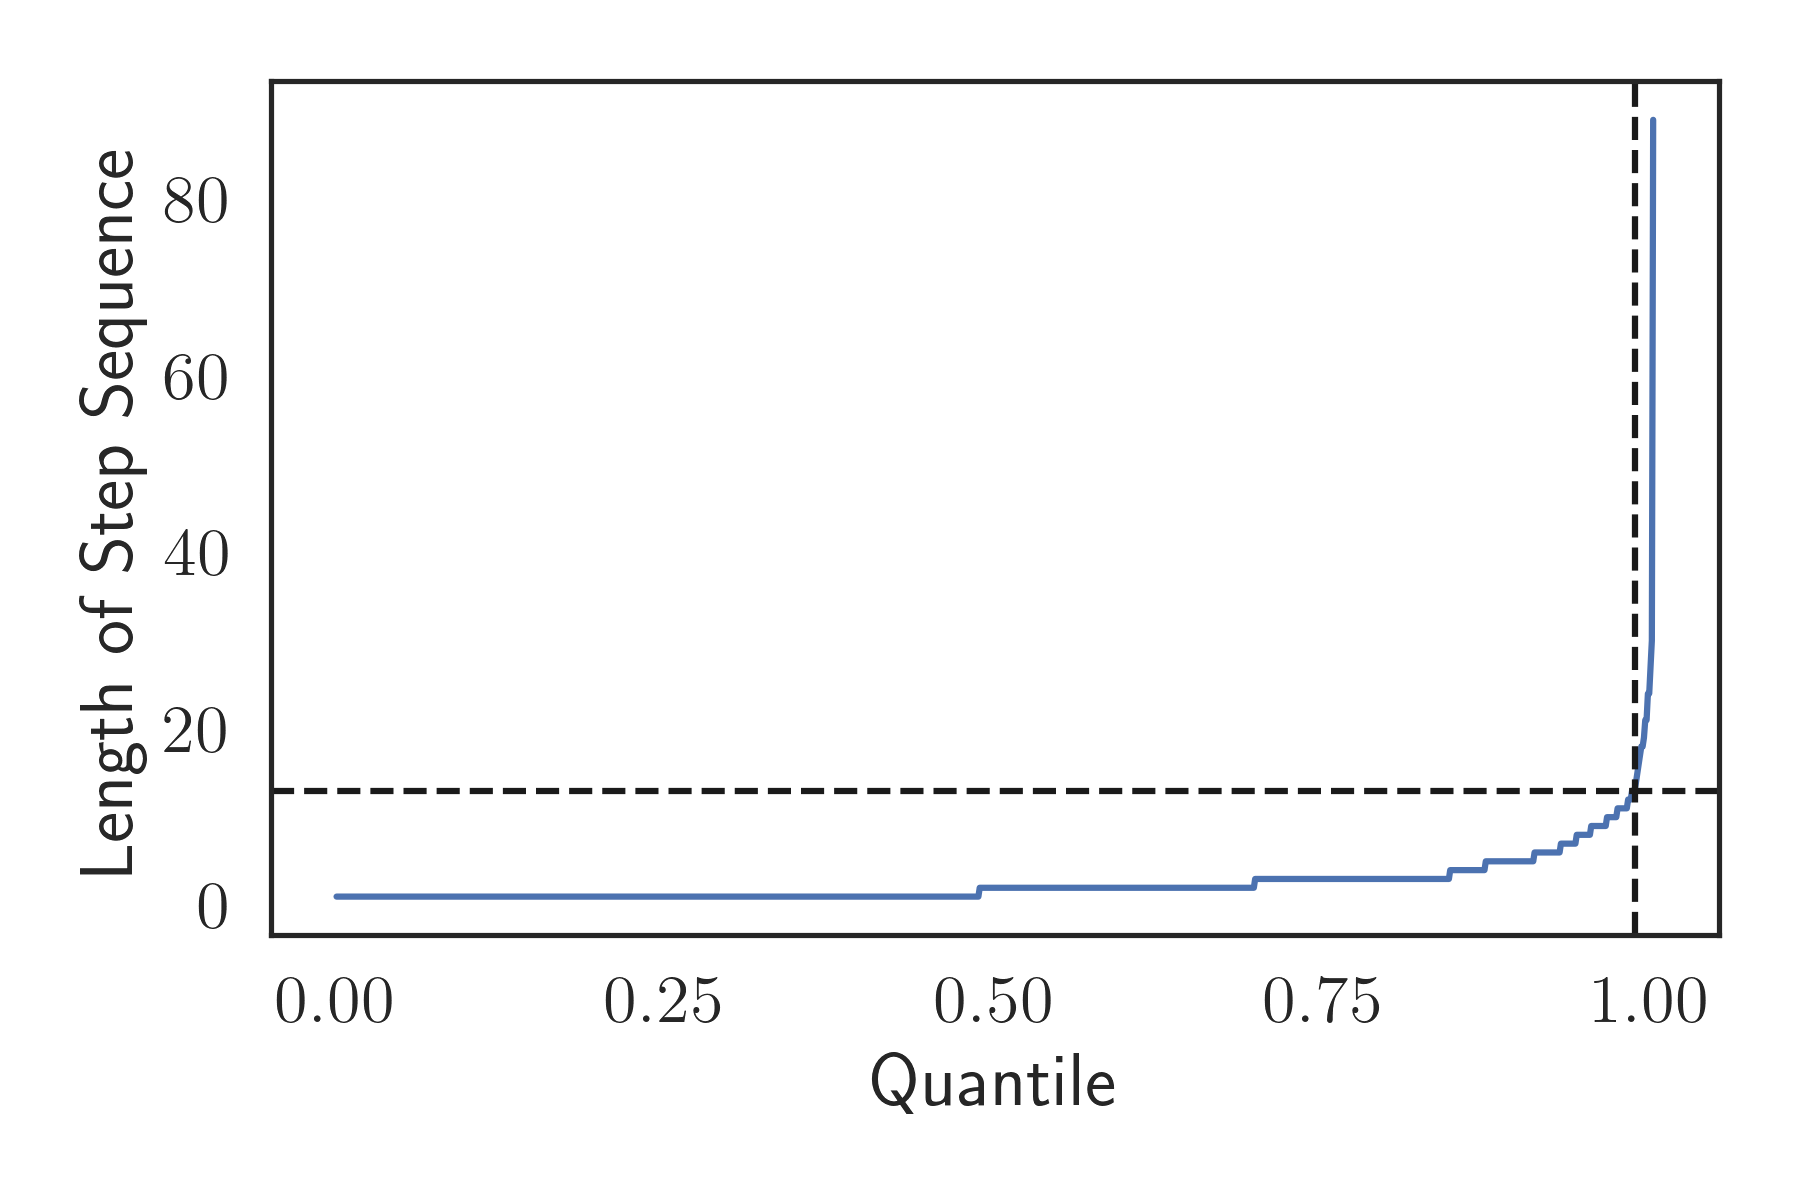
\includegraphics[width=0.6\linewidth]{figures/smells/step-sequences-quantiles.png}
\caption{The blue curve represent the evolution of the length of the sequences of the step as the quantiles increase. The intersection of the black doted lines displays the knee point (0.986, 13) at which the values sequence lengths values start to increase dramatically.}  
\label{fig:step-sequences-quantiles}
\end{figure}


\subsubsection{Middle Man (MM)}

\begin{itemize}
    \item \textbf{Description:} A test component (keyword, macro, function) delegates all its tasks to another test component.

    \item \textbf{Impact on Readability:} The levels of indirection make the test harder to follow by future readers.
    
    \item \textbf{Detection Method:} The principle of delegating is doing nothing and simply calling another function. Thus, we express the count metric, $S_{MM}(t)$, as the number of \emph{User Keywords} called from a test that are composed of a single call to another \emph{Keyword} and the density metric, $D_{MM}(t)$, as the he number of \emph{User Keywords} called from a test that are composed of a single call to another \emph{User Keyword} and the density metric over the total number of \emph{Keyword} called by the test. More formally:
    
    \begin{equation*}
        S_{MM}(t) = \abs{K_{t} \cap K_{delegate}}
    \end{equation*}
    
    \begin{equation*}
        D_{MM}(t) = \frac{\abs{K_{t} \cap K_{delegate}}}{\abs{K_{t}}}
    \end{equation*}
    
    where $\abs{K_{t}}$ is the number of \emph{User Keywords} in a test $t$ and $\abs{K_{t} \cap K_{delegate}}$ is the number of \emph{User Keywords} performing a single call to one other \emph{User Keyword} (we ignore logging action) without performing any subsequent action on their own, \emph{i.e.} \emph{Delegate Keyword}.
    
    \item \textbf{Refactoring Actions:} The symptom is considered refactored if the \emph{Delegate Keyword} call is replaced with another call which is not simply delegating its actions. Thus, we propose the refactoring pattern, $R_{MM}(c)$ where $c$ is a call to a \emph{Delegate Keyword} as:

    \begin{equation*}
        R_{MM}(c) = c_{K_{t, delegate}} \xrightarrow{action} c_{K_{t, \neg delegate}}
    \end{equation*}
    
    where $c_{K_{t, delegate}}$ is a call to a \emph{Delegate Keyword} and $c_{K_{t, \neg delegate}}$ is a call to any \emph{Keyword} not performing delegation.
\end{itemize}

\subsubsection{Missing Assertion (MA)}

\begin{itemize}
    \item \textbf{Description:} The test lacks any explicit assertions.

    \item \textbf{Impact on Readability:} Future readers are left in the potentially frustrating position of puzzling over the intention of the test.
    
    \item \textbf{Detection Method:} The metric detects the absence of call to \emph{Library Keyword} annotated as ``assertion'' within the test. Because the symptom can at most appear once in the test, both the count metric, $S_{MA}(t)$ and the density metric $D_{MA}(t)$ are express as the absence of an assertion call in the test. More formally:
    
    \begin{equation*}
        S_{MA}(t) = D_{MA}(t) = 
        \begin{cases}
            1,   & \text{if } C_{t} \cap C_{assert} = \emptyset\\
            0,   & \text{otherwise}
        \end{cases}
    \end{equation*}
    
    \item \textbf{Refactoring Actions:} The symptom is considered refactored if \emph{Library Keyword} annotated as ``assertion'' is introduced in test that is missing any assertion. Thus, we propose the refactoring pattern, $R_{MA}(t)$, where $t$ is the test lacking any assertion as:
    
    \begin{equation*}
        R_{MA}(t) = \emptyset \xrightarrow{action} c_{t, assertion}
    \end{equation*}
    
    where $c_{t, assertion}$ is a call to a \emph{Library Keyword} annotated as ``assertion'' in a test $t$.
\end{itemize}

\subsubsection{Narcissistic (N)}

\begin{itemize}
    \item \textbf{Description:} The test uses the first person pronoun ``I'' to refer to its actors and does not uniquely qualify those actors.

    \item \textbf{Impact on Readability:} The test is harder to read because it is not clear who ``I'' is and what are the roles that ``I'' has.
    
    \item \textbf{Detection Method:} Using text tagging, we identify calls from the acceptance criteria, \emph{i.e.} ``test steps'', using a personal pronouns as the subject in there name as symptomatic. Furthermore, the implementation used in our experiments supports the different languages present in our dataset (namely, French and English).. Thus, we express the count metric, $S_{N}(t)$, as the number of steps in the acceptance criteria of a test that are using a personal pronoun and the density metric, $D_{N}(t)$, as the number of steps in the acceptance criteria of a test that are using a personal pronoun over the total number of steps in the acceptance criteria of the test:
    
    \begin{equation*}
        S_{N}(t) = \abs{C_{t} \cap C_{step} \cap C_{I}}
    \end{equation*}
    
    \begin{equation*}
        D_{N}(t) = \frac{\abs{C_{t} \cap C_{step} \cap C_{I}}}{\abs{C_{t} \cap C_{step}}}
    \end{equation*}
    
    where  $\abs{C_{t} \cap C_{step}}$ is the number of ``test steps'' for a test $t$ and $\abs{C_{t} \cap C_{step} \cap C_{I}}$ is the number of ``test steps'' using a personal pronouns as the subject in there name.
    
    \item \textbf{Refactoring Actions:} The symptom is considered refactored if the name of a symptomatic ``test steps'' is changed so that it does not contain a personal pronoun anymore. Thus,  we propose the refactoring pattern, $R_{N}(c)$, where $c$ is a step of the acceptance criteria of a test $t$:
    
    \begin{equation*}
        R_{N}(c) = c_{t, step, I} \xrightarrow{action} c_{t, step, \neg I}
    \end{equation*}
    
    where $c_{t, step, I}$ is a \emph{User Keyword} called by a ``test steps'' using the personal pronoun ``I'' as the subject and $c_{t, step, \neg I}$ is the \emph{User Keyword} with its new name not using the personal pronoun ``I'' as the subject. Therefore, a fix is detected only when the name of a \emph{User Keyword} called by a ``test steps'' is changed.
\end{itemize}

\subsubsection{Noisy Logging (NL)}

\begin{itemize}
    \item \textbf{Description:} The test logs the state of the fixtures.

    \item \textbf{Impact on Execution:} There is too much noise in the output from the tests, making its analysis more cumbersome.

    \item \textbf{Detection Method:} In this work, we associate the fixture code to the setup of a test. Thus, we express the count metric, $S_{NL}(t)$, as the number of calls to \emph{Library Keywords} annotated as ``logging'' from the setup of a test and the density metric, $D_{NL}(t)$, as the number of calls to \emph{Library Keywords} annotated as ``logging'' from the setup of a test over the total number of calls from the setup of the test. More formally:

    \begin{equation*}
        S_{NL}(t) = \abs{C_{t} \cap C_{setup} \cap C_{logging}}
    \end{equation*}
    
    \begin{equation*}
        D_{NL}(t) = \frac{\abs{C_{t} \cap C_{setup} \cap C_{logging}}}{C_{t} \cap C_{setup}}
    \end{equation*}
    
    where $\abs{C_{t} \cap C_{setup}}$ is the size of the set of \emph{Library Keyword} called from the setup of a test $t$ and $\abs{C_{t} \cap C_{setup} \cap C_{logging}}$  is the size of the set of \emph{Library Keyword} annotated as ``logging'' called from the setup of test $t$.
    
    \item \textbf{Refactoring Action:} The symptom is considered refactored if the call to the \emph{Library Keyword} annotated as ``logging'' called from the setup of test $t$, $c_{t, setup, log}$, is removed. Thus we propose the refactoring pattern, $R_{NL}(c)$, performed on a \emph{Keyword} call $c$ as follow:
    
    \begin{equation*}
        R_{NL}(c) = c_{t, setup, log} \xrightarrow{action} \emptyset
    \end{equation*}
    
    Note that removing a parent of $c_{t, setup, log}$ is not considered as fixing the smell.
\end{itemize}

\subsubsection{Obscure Test (OT)}

\begin{itemize}
    \item \textbf{Description:} The test behavior is difficult to understand because the test does not clearly state what it is verifying. Typical symptoms are hardcoded values, high cyclomatic complexity and/or function or procedure calls with high number of parameters.

    \item \textbf{Impact on Readability:} Future reader might not understand the meaning of a hardcoded value, hence, missing the intention of the test. As with a high cyclomatic complexity it becomes hard for the future reader to follow the execution flow of the test and grasp what it is doing.
    
    \item \textbf{Impact on Maintenance:} It is difficult to determine where to perform changes if hardcoded values are scattered all over the test code. Furthermore, test with high cyclomatic complexity might have side effect overseen during maintenance which might lead to future problems.
    
    \item \textbf{Detection Method:} In this work, we focus on one of the expression of an obscure test: the overuse of hardcoded values. The code starts to smell when hardcoded values are used directly in calls to both \emph{User Keyword} and \emph{Library Keywords}, instead of relying on variables. Thus, we express the count metric, $S_{OT}(t)$, as the number of hardcoded arguments present in a test and the density metric $D_{OT}(t)$ as the number of hardcoded arguments present in the test over the total number of arguments from that test. More formally:
    
    \begin{equation*}
        S_{OT}(t) = \abs{A_{t} \cap A_{hardcoded}}
    \end{equation*}
    
    \begin{equation*}
        D_{OT}(t) = \frac{\abs{A_{t} \cap A_{hardcoded}}}{\abs{A_t}}
    \end{equation*}
    
    where $\abs{A_t}$ is the size of the set of arguments passed to \emph{Keyword} calls in a test $t$ and $\abs{A_{t} \cap A_{hardcoded}}$ is the size of the set of arguments passed to \emph{Keyword} calls which are hardcoded.
    
    \item \textbf{Refactoring Actions:} Focusing on hardcoded values, the symptom is considered refactored if an argument passed to \emph{Keyword} call as a hardcoded value is replaced by a variable. Thus, we propose the refactoring pattern, $R_{OT}(a)$, where $a$ is a \emph{Keyword} call arguments as:
    
    \begin{equation*}
        R_{OT}(v) = a_{t, hardcoded} \xrightarrow{action} a_{t, variable}
    \end{equation*}
    
    where $a_{t, hardcoded}$ is a hardcoded \emph{Keyword} call argument and $a_{t, variable}$ is a variable \emph{Keyword} call argument.
\end{itemize}

\subsubsection{On the Fly (OtF)}

\begin{itemize}
    \item \textbf{Description:} The test calculates an expected results during its execution instead of relying on pre-computed values.

    \item \textbf{Impact on Readability:} By embedding the business rule in the assertion, the code for the automated test can become as complicated as the system under test.
    
    \item \textbf{Detection Method:} The expected value should be a constant or a reference to a constant and not computed during the test. Thus, we express the count metric, $S_{OtF}(t)$, as the number of expected values that are computed in the test and the density metric, $D_{OtF}(t)$, as the number of expected arguments from assertion calls that are computed in the test over the total number of expected arguments from assertion calls:
    
    \begin{equation*}
        S_{OtF}(t) = \abs{A_{t} \cap A_{expected} \cap A_{computed}}
    \end{equation*}
    
    \begin{equation*}
        D_{OtF}(t) = \frac{\abs{A_{t} \cap A_{expected} \cap A_{computed}}}{\abs{A_{t} \cap A_{expected}}}
    \end{equation*}
    
    where $\abs{A_{t} \cap A_{expected}}$ is the number of ``expected'' arguments in calls to \emph{Library Keywords} annotated as ``assertion'' for a test $t$ and  $\abs{A_{t} \cap A_{expected} \cap A_{computed}}$ is the number of ``expected'' arguments in calls to \emph{Library Keywords} annotated as ``assertion'' resolved during the execution of the test $t$. Note that the identification of the ``expected'' argument is based on the definition of the \emph{Library Keyword}. When a \emph{Library Keyword} annotated as ``assertion'' contains a field called ``expected'', it is considered by the engine as the placeholder for the expected value. For instance, the library keyword \emph{Should be equal} from the Builtin library takes six arguments: \emph{value}, \emph{expected}, \emph{message}, \emph{values}, \emph{ignore\_case} and \emph{formatter}. Hence, in this case the expected argument is the second one.
    
    \item \textbf{Refactoring Action:} The symptom is considered refactored when the assertion is preserved but the expected value is not computed on the fly. This leads to the following equation for a refactoring action, $R_{OtF}$, addressing a symptom in an argument $a$:
    
    \begin{equation*}
        R_{OtF}(a) =  a_{t, expected, computed} \xrightarrow{action} a_{t, expected, \neg computed}
    \end{equation*}
    
    where $a_{t, expected, computed}$ is an expected value that is computed on the fly and $a_{t, expected, \neg computed}$ is an expected value that is not computed on the fly, being either hardcoded or provided through a variable pointing to a static value. Thus removing the assertion would not be considered as removing the symptom since $a_{t, expected, \neg computed}$ would not be present.
\end{itemize}

\subsubsection{Over-Checking (OC)}

\begin{itemize}
    \item \textbf{Description:} The test performs some assertions that are not relevant for its scope.

    \item \textbf{Impact on Readability:} It becomes harder to understand what is the main intent of the test. Many assertions suggests the test is checking many different properties.
    
    \item \textbf{Impact on Maintenance:} The test may be too sensitive to the evolution of the \gls{sut}, verifying implementation properties instead of behavioral ones.
    
    \item \textbf{Detection Method:} As the ratio assertions to actions on \gls{sut} increases, the chances that all the assertions are relevant decreases. Thus we express the count metric, $S_{OC}(t)$, as the number of assertions in a test and the density metric, $N_{OC}(t)$, as the number of assertions in a test over the total number of calls in the test. More formally:
    
    \begin{equation*}
        S_{OC}(t) = \abs{C_{t} \cap C_{assertion}}
    \end{equation*}
    
    \begin{equation*}
        N_{OC}(t) = \frac{ \abs{C_{t} \cap C_{assertion}}}{\abs{C_{t}}}
    \end{equation*}
    
    where $\abs{C_{t}}$ is the size of the set \emph{Library Keywords} calls and $\abs{C_{t} \cap C_{assertion}}$ is the size of the set of calls to \emph{Library Keywords} annotated as ``assertion''.
    
    \item \textbf{Refactoring Actions:} The symptom is considered refactored if the call to a \emph{Library Keyword} annotated with ``assertion'', $c_{t, assertion}$ , is removed from a test $t$. Thus, we propose the refactoring pattern, $R_{OC}(c)$ where $c$ is a call to an \emph{Library Keyword} annotated with ``assertion'' as:
    
    \begin{equation*}
        R_{OC}(c) = c_{t, assertion} \xrightarrow{action} \emptyset
    \end{equation*}
\end{itemize}

\subsubsection{Sensitive Locators (SL)}

\begin{itemize}
    \item \textbf{Description:} The test uses element identification selectors that have long chains to identify an element in the user interface. e.g. complex x-pass or CSS selector for web application.

    \item \textbf{Impact on Maintenance:} This leads to fragile tests, as any change in that chain from the user interface representation will break the tests.
    
    \item \textbf{Detection Method:} The complexity of a locator can be expressed by how deep the locator needs to go in the hierarchy of the UI, be it an x-pass, a CSS selector or any UI representation based on a hierarchy. A locator, $A_{locator}$, can be expressed as the number of \gls{gui} element, $\abs{E}$, that have to be traversed to uniquely locate the target \gls{gui} element. Thus, we express the count metric, $S_{SL}(t)$, as the number of locator arguments that visit more than one \gls{gui} elements and the density metric, $D_{SL}(t)$, the number of of locator arguments that visit more than one \gls{gui} elements in a test over the total number of locator arguments present in the test. More formally:
    
    \begin{equation*}
        S_{SL}(t) = \abs{A_t \cap A_{locator} \cap A_{\abs{E} > 1}}
    \end{equation*}
    
    \begin{equation*}
        D_{SL}(t) = \frac{\abs{A_t \cap A_{locator} \cap A_{\abs{E} > 1}}}{\abs{A_t \cap A_{locator}}}
    \end{equation*}
    
    where $\abs{A_t \cap A_{locator} \cap A_{\abs{E} > 1}}$ is the number of locators that require to visit more than one element $E$ of the \gls{gui} to be uniquely identified (\emph{e.g.} the XPath ``/html/body/div[4]/button'' visits 4 elements to quality the button where the XPath ``//button[@id ="unique-id"]'' only needs to visit one element). Note that Robot Framework using dynamic types, only \emph{Library Keyword} calls explicitly specify a type for their parameters. Therefore, for each \emph{Library Keyword} call requiring a locator as an argument, the engine resolve all the values possible for the argument within the test to populate the set $A_{locator}$.
    
    \item \textbf{Refactoring Actions:} The symptom is considered refactored if the value of a node $l$ flagged as complex locator sees its length go down to one. Thus, we propose the refactoring pattern, $R_{SL}(l)$, as follow:
    
    \begin{equation*}
        R_{SL}(c) = l_{\abs{E} > 1} \xrightarrow{action} l_{\abs{E} = 1}
    \end{equation*}
    
    where $l_{\abs{E} > 1}$ is a node defining the value of a sensitive locator and $l_{\abs{E} = 1}$ is the same node but with a simple locator expression. Note that a change is only accounted for when the value of the locator is modified.
\end{itemize}

\subsubsection{Sneaky Checking (SC)}

\begin{itemize}
    \item \textbf{Description:} The test hides its assertions in actions that are at the wrong level of details.

    \item \textbf{Impact on Readability:} The future reader is not able to understand what is being tested by just looking at the main steps of the acceptance criteria without a need to inspect how low level details are implemented.
    
    \item \textbf{Detection Method:} A \emph{User Keyword} only calling an \emph{Library Keyword} annotated as ``assertion'' can be seen as hiding the assertion to the callers of that \emph{User Keyword}. Thus, we express the count metric, $S_{SC}(t)$, as the number of unique \emph{User Keywords} called by a test and only calling an assertion and the density metric, $D_{SC}(t)$, as the number of unique \emph{User Keywords} called by the test and only calling an assertion over the number of unique \emph{User Keywords} called by that test. More formally:
    
    \begin{equation*}
        S_{SC}(t) = \abs{K_{t} \cap K_{assert}}
    \end{equation*}
    
    \begin{equation*}
        D_{SC}(t) = \frac{\abs{K_{t} \cap K_{assert}}}{\abs{K_{t}}}
    \end{equation*}
    
    where $\abs{K_{t}}$ is the total number of unique \emph{User Keywords} and $\abs{K_{t} \cap K_{assert}}$ is the number of \emph{User Keywords} only calling an \emph{Library Keyword} annotated as ``assertion'' (logging actions are ignored).
    
    \item \textbf{Refactoring Actions:} The symptom is considered refactored if a \emph{User Keywords} only calling a \emph{Library Keyword} annotated as ``assertion'', $k_{t, assert}$, is removed from the test $t$. Thus, we propose the refactoring pattern, $R_{SC}(k)$, where $k$ is a \emph{User Keywords} as:
    
    \begin{equation*}
        R_{SC}(k) = k_{t, assert} \xrightarrow{action} \emptyset
    \end{equation*}
\end{itemize}

\subsubsection{Stinky Synchronization (SS)}

\begin{itemize}
    \item \textbf{Description:} The test fails to use proper synchronization points with the system under test.

    \item \textbf{Impact on Execution:} The test becomes oversensitive to the response time, leading to flaky tests, or very slow tests when choosing very conservative wait points.
    
    \item \textbf{Detection Method:} This symptom is associated with the use of explicit and fixed synchronization, independent from the \gls{sut} such as a pausing the test for a specific amount of time. Thus, we express the count metric, $S_{SS}(t)$, as the number of calls to explicit pause from a test and the density metric, $D_{SS}(t)$, as the number of calls to explicit pause from a test over the total number of synchronization calls. More formally:
    
    \begin{equation*}
        S_{SS}(t) = \abs{C_{t} \cap C_{sync} \cap C_{sleep}}
    \end{equation*}
    
    \begin{equation*}
        D_{SS}(t) = \frac{\abs{C_{t} \cap C_{sync} \cap C_{sleep}}}{\abs{C_{t} \cap C_{sync}}}
    \end{equation*}
    
    where $\abs{C_{t} \cap C_{sync}}$ is the size of the set of calls to \emph{Library Keyword} annotated as ``synchronization'' in a test $t$ and $\abs{C_{t} \cap C_{sync} \cap C_{sleep}}$ is the size of the set of calls to \emph{Library Keyword} annotated as ``synchronization'' by pausing the test execution for a specified amount of time. In the case of Robot Framework, it is instantiated by calls to the \emph{Library Keyword} ``Sleep''.
    
    \item \textbf{Refactoring Actions:} The symptom is considered refactored if a \emph{Library Keyword} call annotated as ``synchronization'' which pausing the test execution of the test for a specified amount of time, $c_{t,sync,sleep}$, is removed or replaced by another \emph{Library Keyword} call annotated as ``synchronization'', $c_{t,sync, \neg sleep}$. Thus, we propose two refactoring patterns, $R_{SS, 1}(c)$ and $R_{SS, 2}(c)$, as follow:
    
    \begin{equation*}
        R_{SS, 1}(c) = c_{t,sync,sleep} \xrightarrow{action_1} \emptyset
    \end{equation*}
    
    \begin{equation*}
        R_{SS,2}(c) = c_{t,sync,sleep} \xrightarrow{action_2} c_{t,sync, \neg sleep}
    \end{equation*}
\end{itemize}

\subsection{RQ2: SUIT Smells Distribution}
\label{sec:results-smells-diffusion}

\begin{figure}
\centering
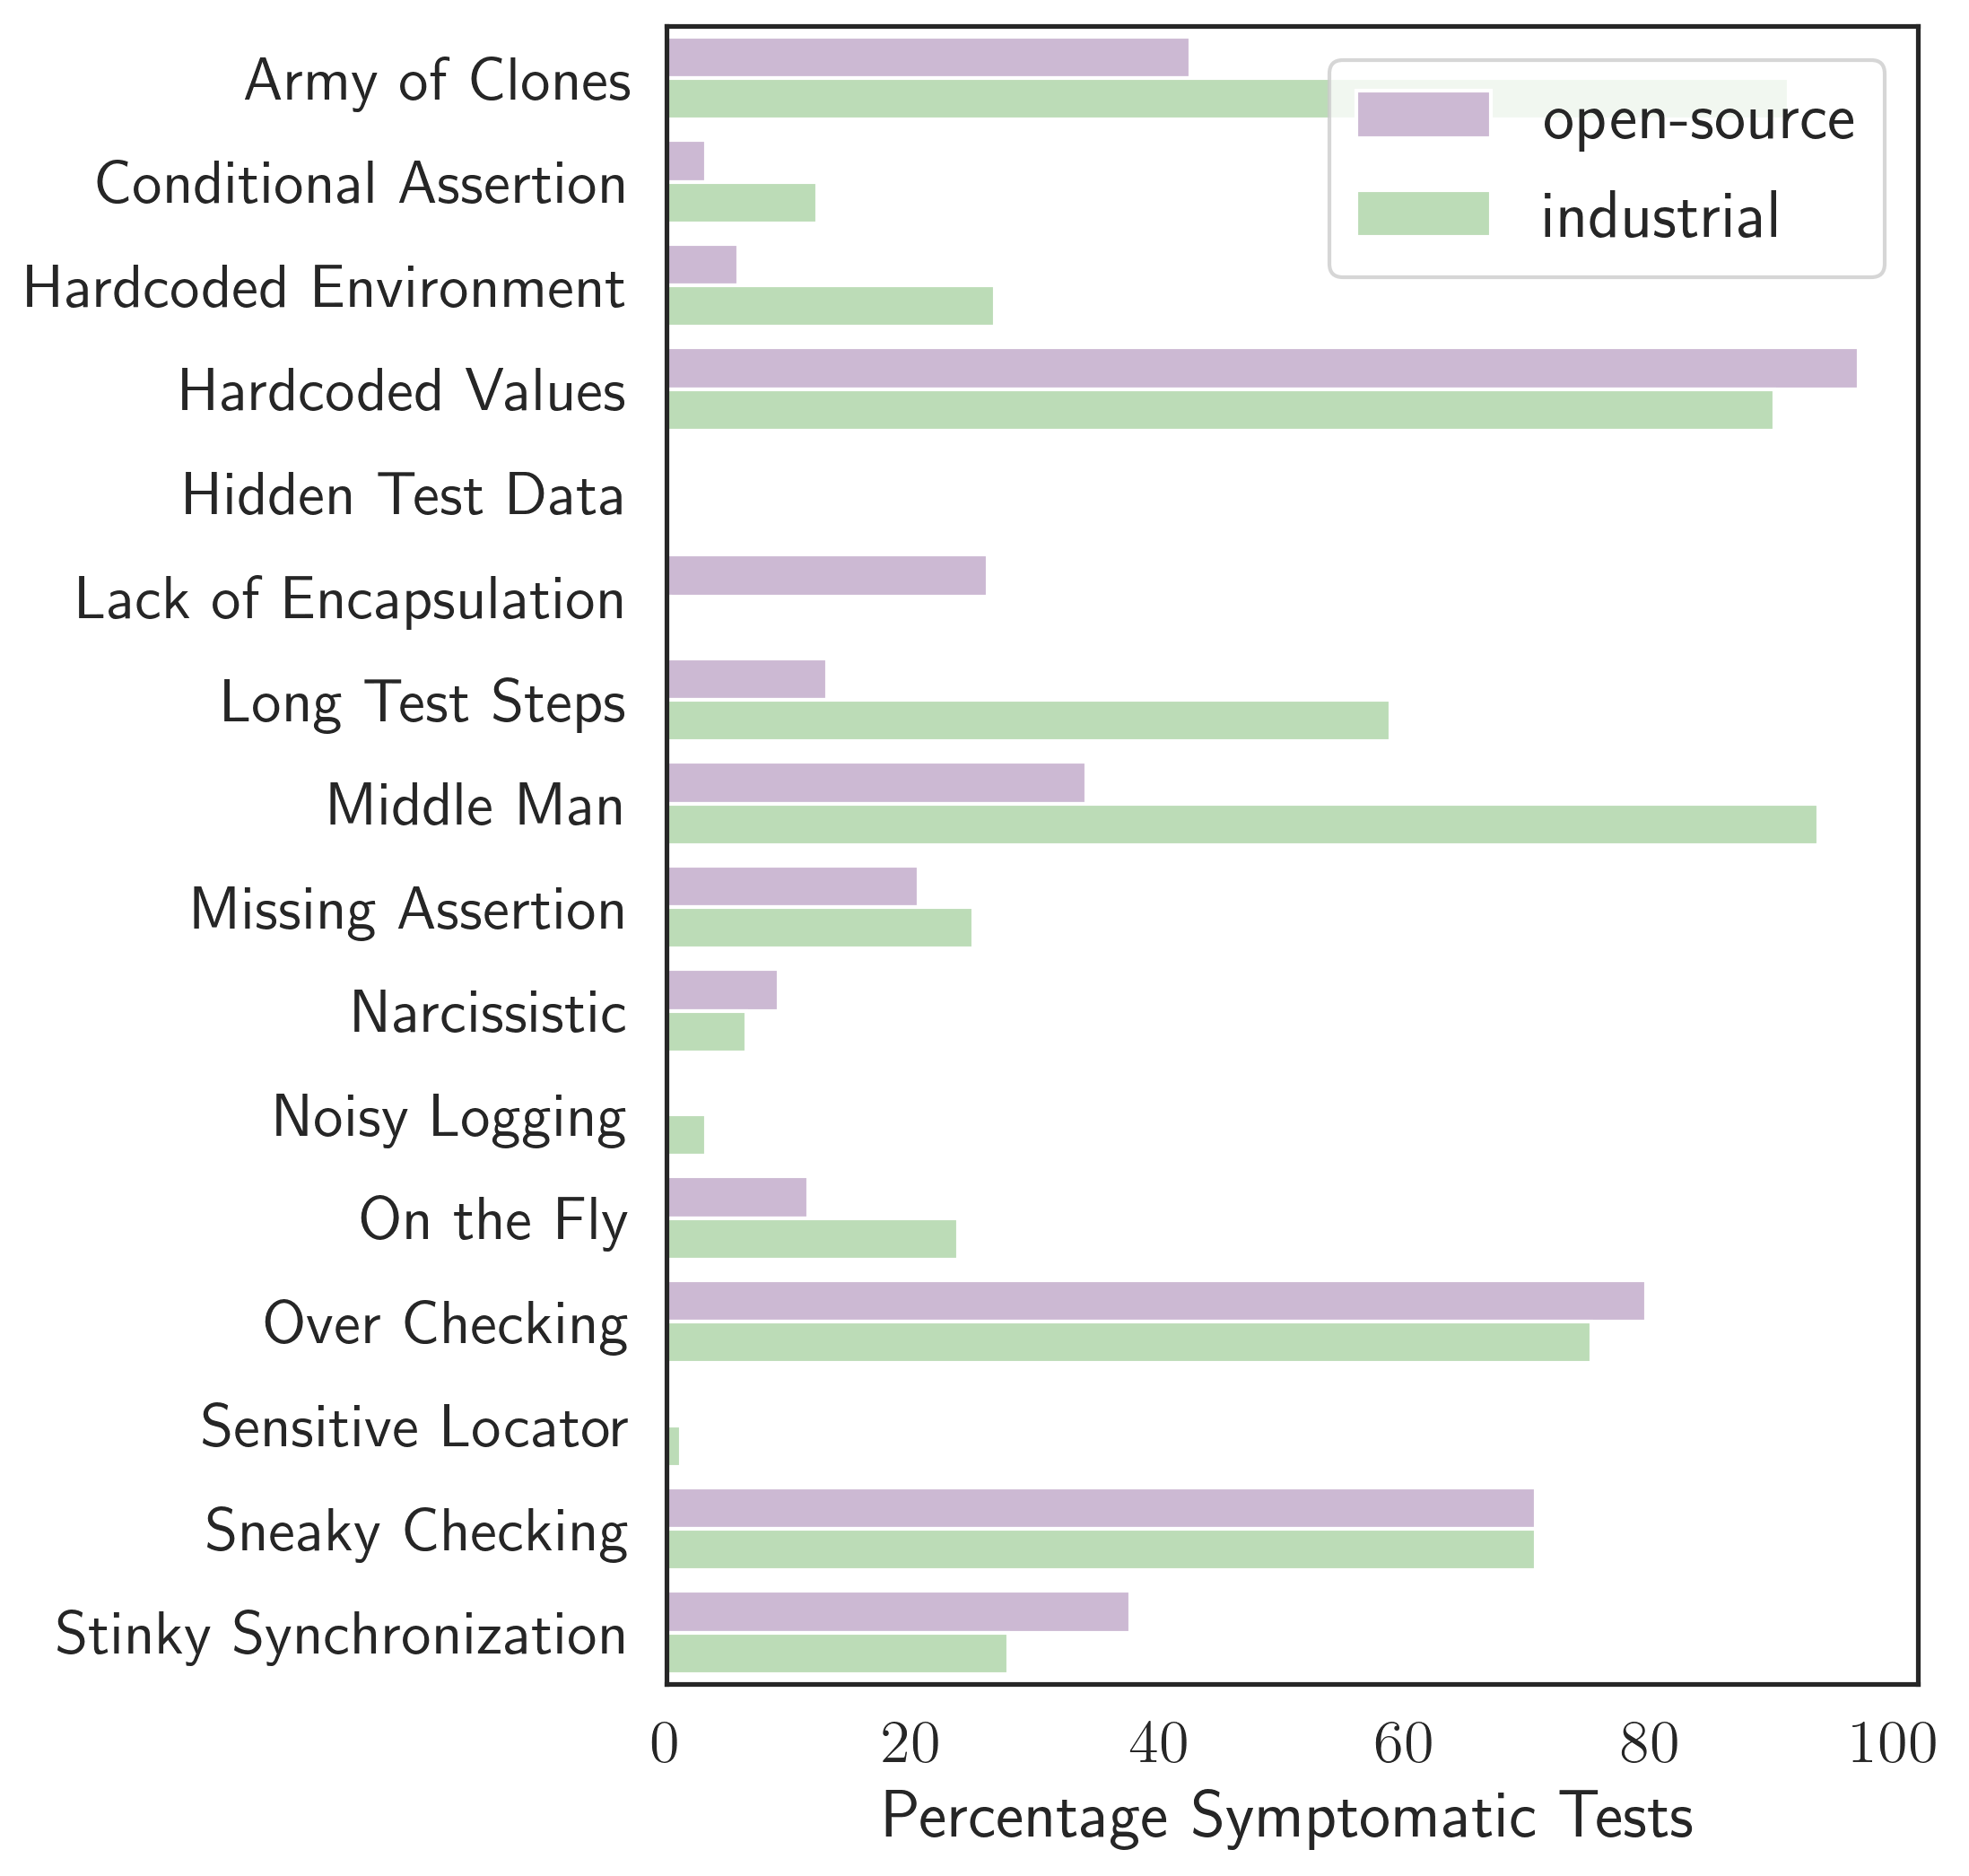
\includegraphics[width=0.9\linewidth]{figures/smells/diffusion.png}
\caption{Percentage of tests exhibiting at least one instance of the symptom for open-source projects and industrial projects.}  
\label{fig:diffusion}
\end{figure}

Building on the metrics derived in Section~\ref{sec:results-smells-catalog}, we show for all projects the number of test exhibiting at least one instance of a symptom in Figure~\ref{fig:diffusion}. The symptom \emph{Hidden Test Data} does not appear neither in open-source project nor in industrial projects. Furthermore, symptoms \emph{Noisy Logging}, \emph{Sensitive Locator}, \emph{Narcissistic} and \emph{HardCoded Environment} manifest in less than 10\% of the tests in open-source and industrial \gls{suit} suites. 

On the other end of the spectrum, three symptoms appear in the majority of the \gls{suit}s: the symptom \emph{Hardcoded Values} appears in more than 90\% in both type of projects, \emph{Over Checking} between 75\% (industrial) and 79.5\% (open-source), and finally \emph{Sneaky Checking} appearing in 70\% of the test in both projects.

Finally, an interesting observation concerns the presence of significant difference between industrial and open-source projects. Notably, at BGL BNP Paribas, three symptoms appear much more often than in open-source projects, namely, \emph{Middle Man} (93.5\%), \emph{Army of Clones} (91.2\%) and \emph{Long Test Steps} (58.8\%). The results for the \emph{Army of Clones} and \emph{Middle Man} can be explained by the structure of the projects at BGL BNP Paribas. Symptoms for the \gls{suit} smell \emph{Army of Clones} are appearing because many repositories are interconnected, leading to code duplication across projects because testers working on different applications or different parts of the system test common functionalities over and over. As for the symptoms of \emph{Middle Man}, their presence is explained by the use of \emph{Keywords} that act as translation layers. While two test steps can perform the same concrete actions on the \gls{sut}, in different context they might operate on a different business logic. Thus, the developers created translation layers to unify the vocabulary used in the acceptance layer of each test. These translation layers are implemented by the use of a \emph{Keyword} only calling one other \emph{Keyword} with a different name. Finally, \emph{Long Test Step} originates from the complex business logic that is expressed by the step in a test at BGL BNP Paribas and is more related to the \gls{sut} and the vocabulary employed by the business analysts than the test suite itself.

\begin{figure}
\centering
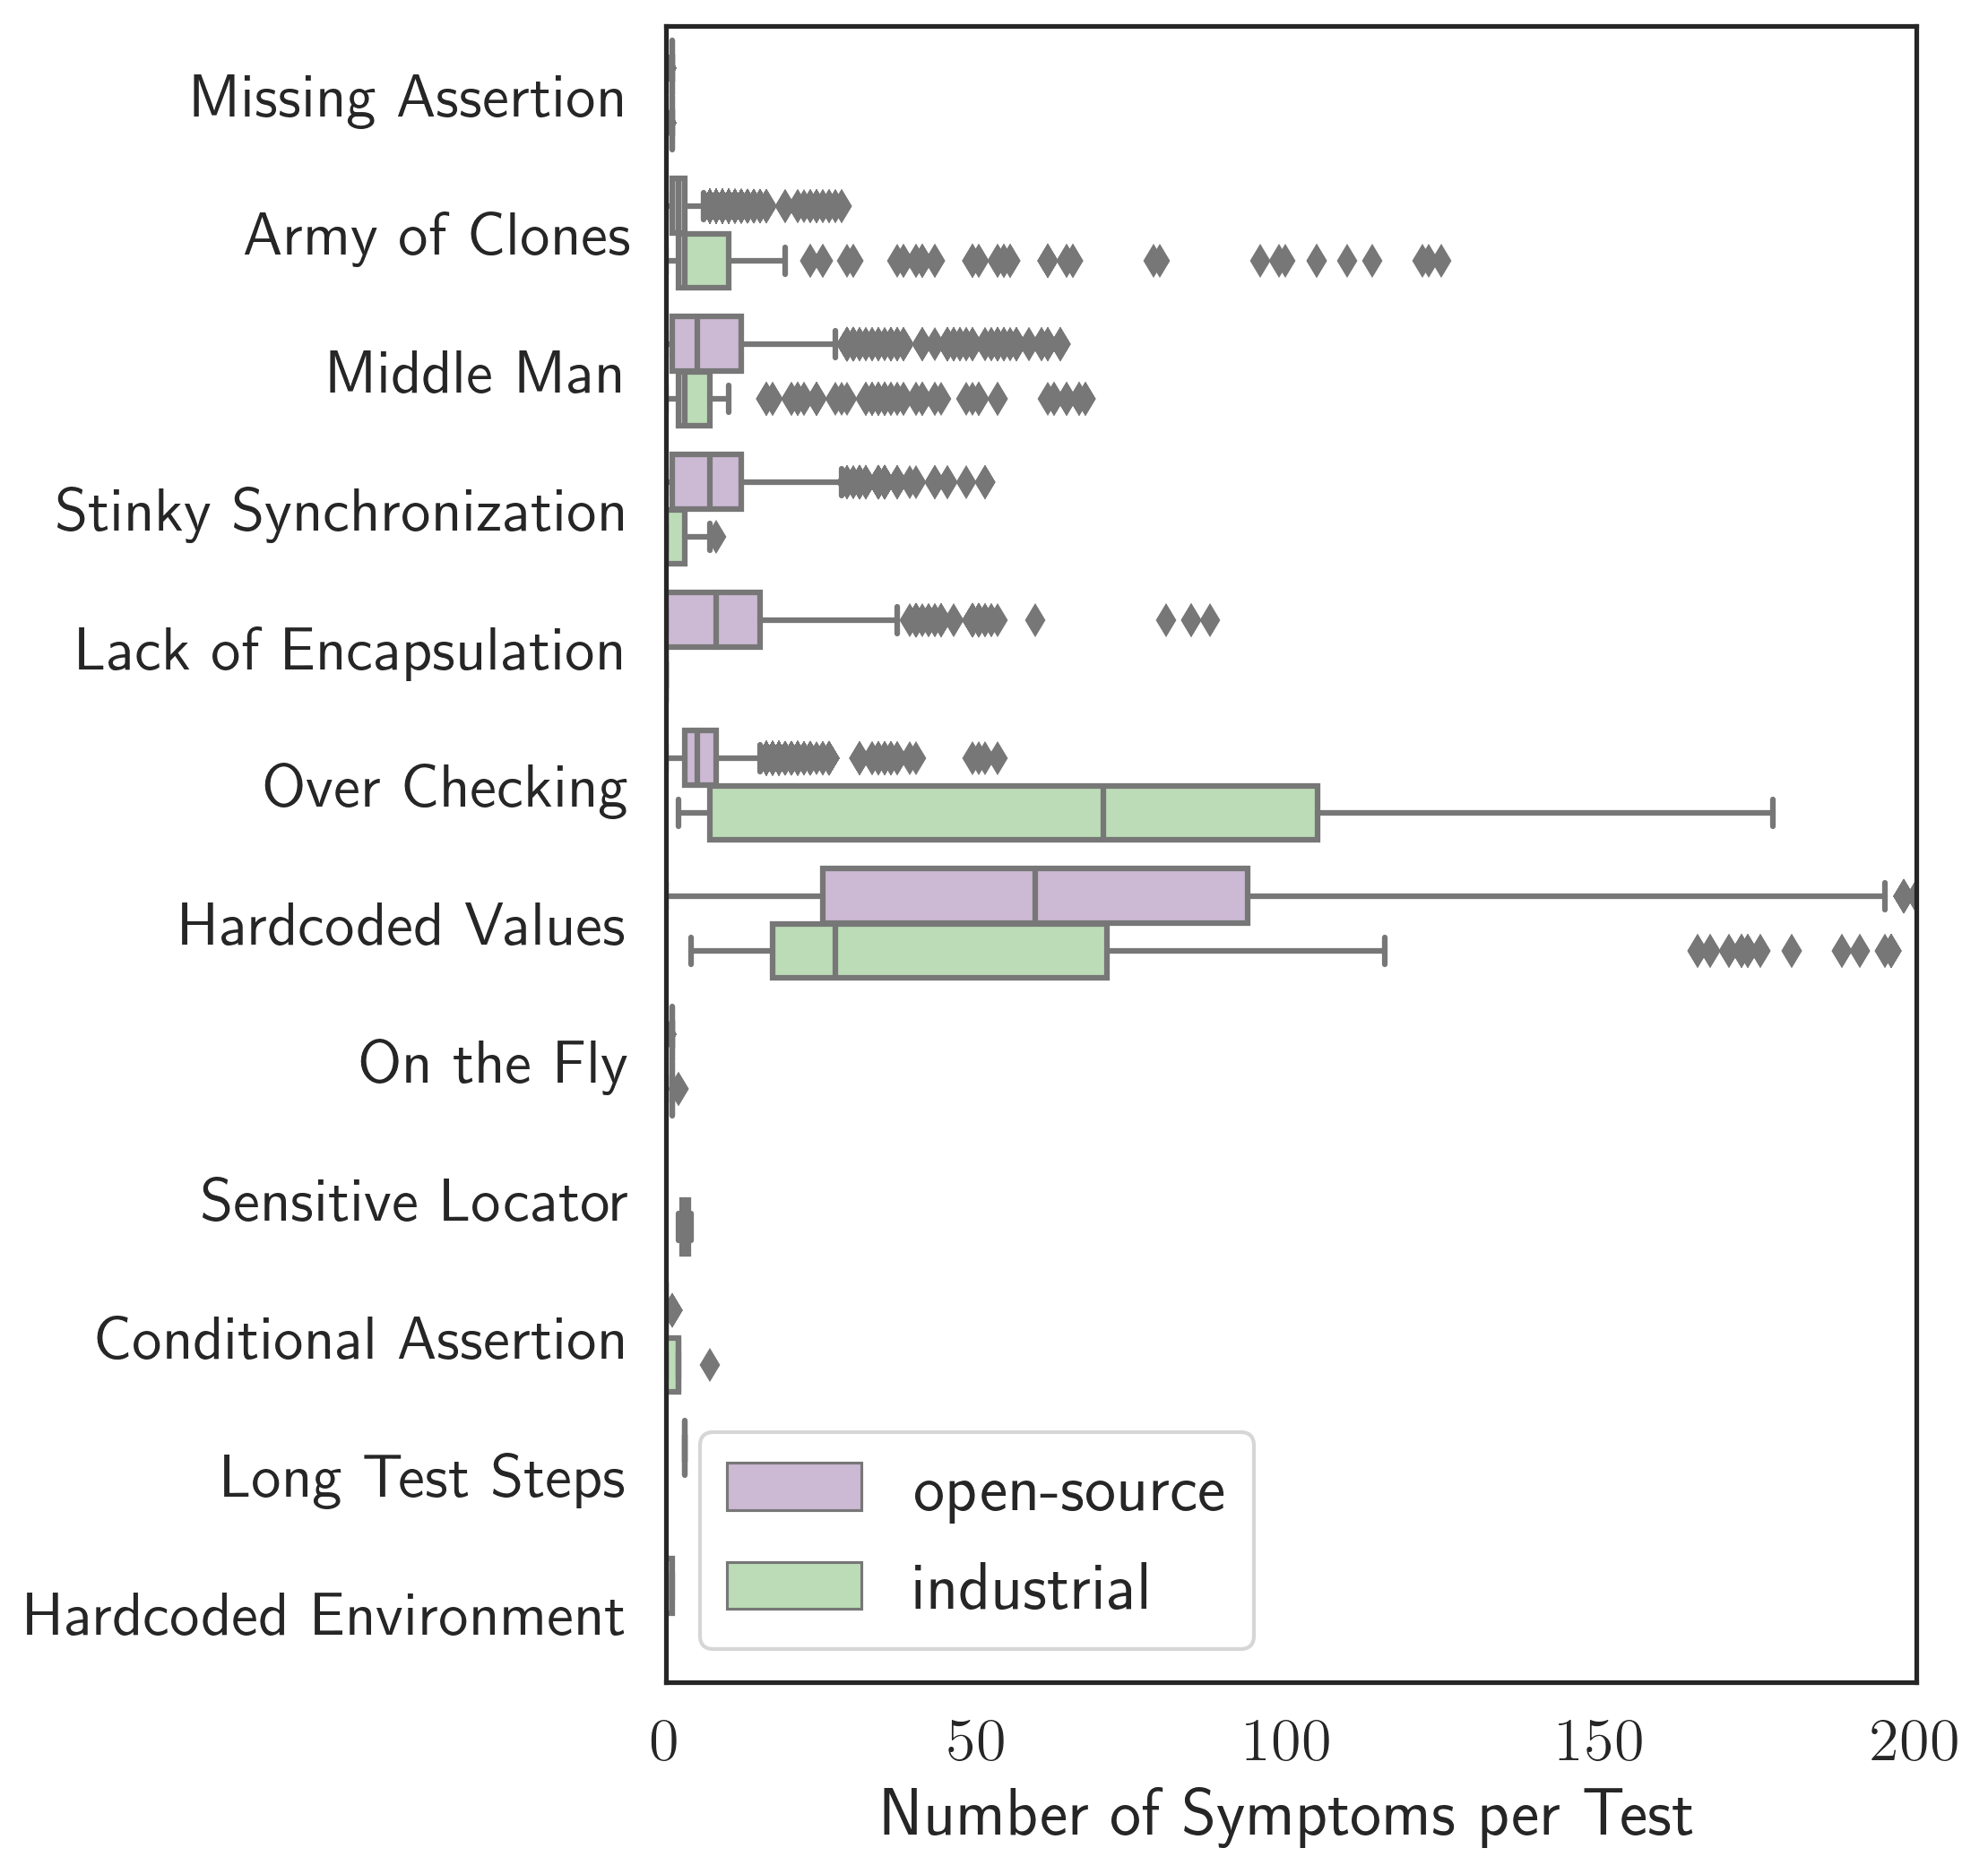
\includegraphics[width=0.9\linewidth]{figures/smells/smell-raw-value-200-distribution-boxplot.png}
\caption{Distribution of the number of symptoms in symptomatic tests for all projects across commits.}  
\label{fig:raw-smells-distribution}
\end{figure}

We continue our analysis with the evaluation of the number of symptoms appearing per tests (Figure~\ref{fig:raw-smells-distribution}). Note that only tests presenting at least one symptom are taken into account in our analysis, \emph{i.e.} symptomatic tests. Looking at \emph{Hardcoded Values}, we see that even both industrial and open-source projects exhibit the same proportion of test containing \emph{Hardcoded Values}, the number varies significantly from a median of 27 in the case of industrial projects to 59 for open-source projects. A similar observation can be made for the case of \emph{Over Checking} where the median varies from 5 (open-source) to 70 (industrial). Finally, the last significant difference regards the symptom \emph{Army of Clones}. Not only the number of test containing duplicated code (Figure~\ref{fig:diffusion}) is higher, but the number of duplicated \emph{Keywords} in symptomatic tests are higher in industrial projects (3 duplicated \emph{Keywords} per test) than in open-source projects (2 duplicated \emph{Keywords} per test).

\begin{figure}
\centering
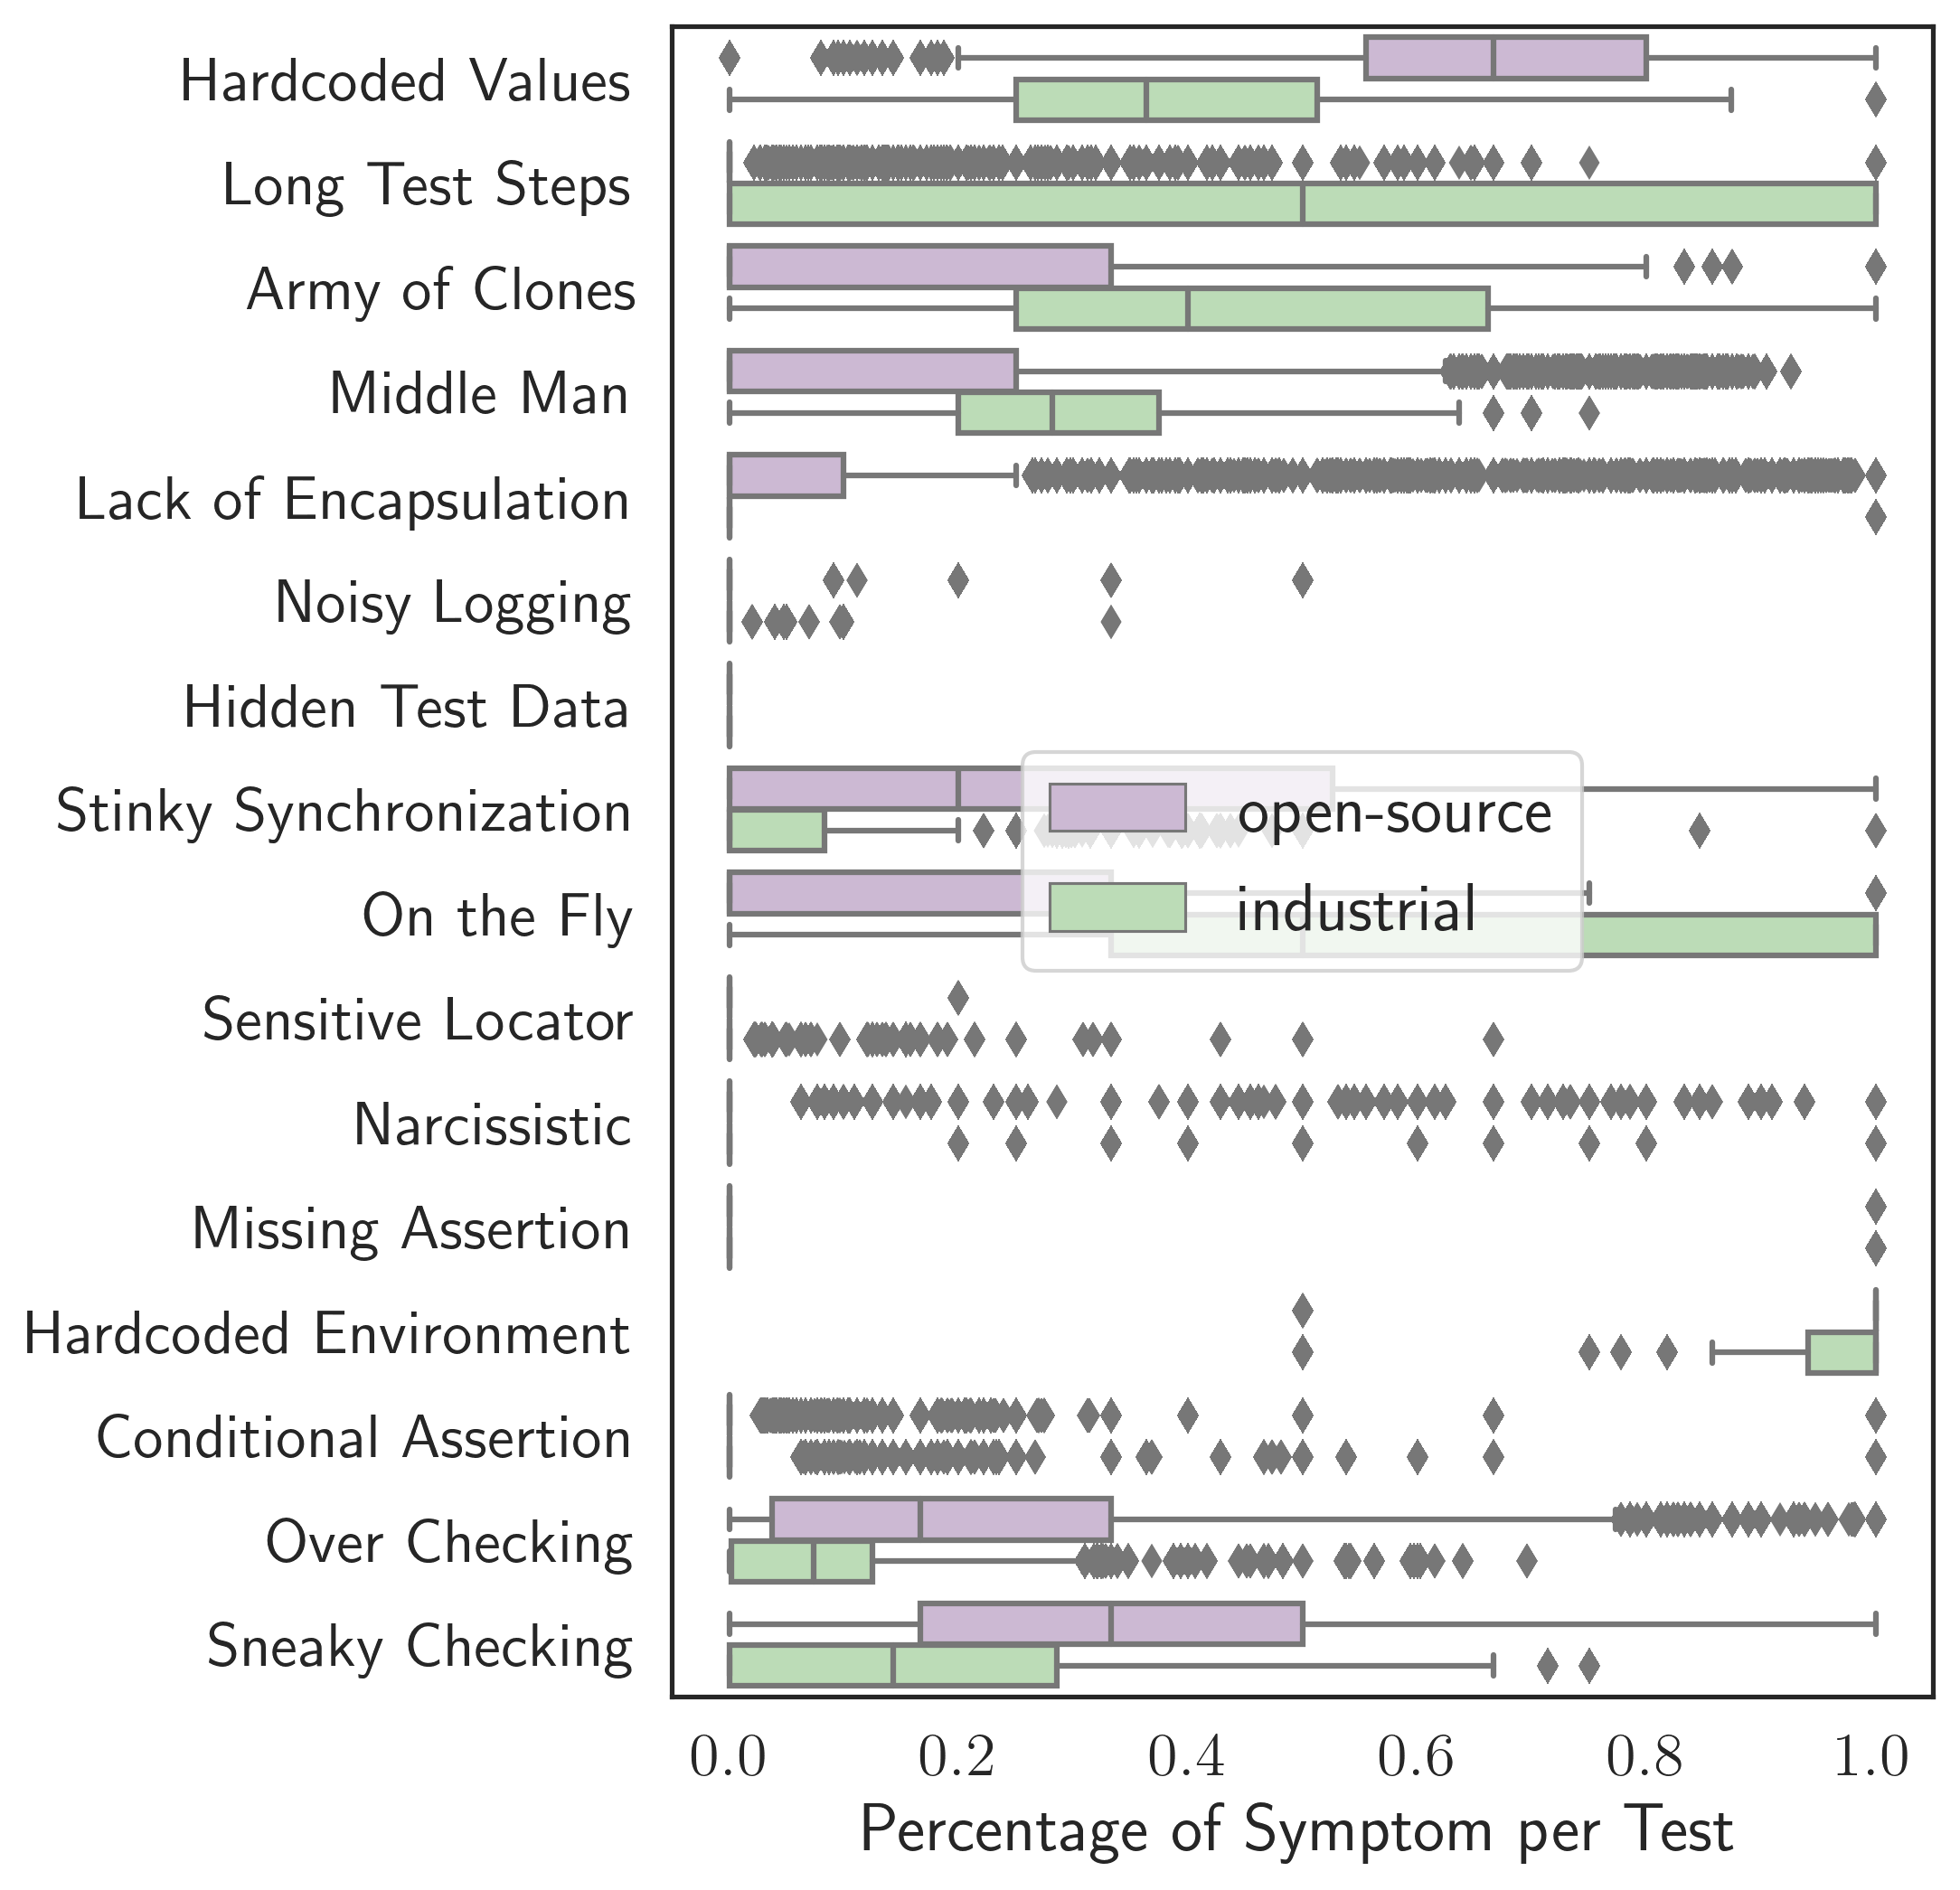
\includegraphics[width=0.9\linewidth]{figures/smells/smell-normalized-distribution-boxplot.png}
\caption{Distribution of the density of symptoms in each test for all projects across commits where the density is the percentage of locations that a symptom could appear at which actually exhibit the symptom.}  
\label{fig:normalized-smells-distribution}
\end{figure}

To put the results of Figure~\ref{fig:raw-smells-distribution} into perspective, we show the density metrics, $D_s(t)$, in Figure~\ref{fig:normalized-smells-distribution}. As a reminder, the density value presents the number of symptoms appearing in a \gls{suit} divided by the number of times it could have appeared. One interesting finding to put in contrast with the previous figure regards the smell \emph{Hardcoded Environment}. While the symptoms do not appear often (only outliers present a value greater than 0 in Figure~\ref{fig:raw-smells-distribution}), whenever an environment variable is used, it will generally be through the use of a hardcoded value which is shown by a median value for its density metric at 1 for both open-source and industrial projects. That is, with regard to its potential occurrences, the \gls{suit} smell \emph{Hardcoded Environment} is actually very frequent.

On the other hand, the smells \emph{Noisy Logging}, \emph{Hidden Test Data}, \emph{Sensitive Locator}, \emph{Narcissistic} and \emph{Conditional Assertion} present low scores in the density value. This means that even when the conditions for their occurrence are present, the symptoms  of these smells do not manifest.

%TODO: Ask BGL if they clearly see those smells as a problem.

To assess its potential to appear in a test suite, we consider a symptom as frequent if the median value of the density metric is greater than 0. Thus, \emph{Hardcoded Values} with median values of 0.67 and 0.33, \emph{Over Checking} with median values of 0.17 and 0.08, and \emph{Sneaky Checking} with median values of 0.33 and 0.14, for open-source and industrial projects respectively, are frequent in both industrial and open-source projects. This aligns with the observations from  the count metric and confirms the prevalence of these smells. Similarly, following the same trend from Figure~\ref{fig:raw-smells-distribution} \emph{Army of Clones} (median value of 0.40), \emph{Long Test Step} (median value of 0.5) and \emph{Middle Man} (median value of 0.29) appear often in industrial projects.

Nonetheless, in the case of the industrial project, we observe that \emph{On the Fly} with a median value of 0.67 shows a deviation from the count metric, $S_s(t)$. 
As for open-source projects, we observe that \emph{Sticky Synchronization} is frequent, with a median value of 0.2. The divergence with the count metric can be explained by the fact that many tests do not use explicit synchronization mechanism, thus, limiting the number of tests where the symptom could appear. Furthermore, the difference from the industrial project can explained by the hard policy in the QA team at BGL BNP Paribas, where explicit timeouts are considered as a major source of flakiness. Indeed, explicit timeouts are strongly discouraged by the QA team and are usually removed during code reviews.

BGL BNP Paribas and the open-source projects present similar trends despite their difference in terms of design and architecture. We observe that 7 out of the 16 smells symptoms do not typically appear in \gls{suit}s, whereas the smells \emph{Hardcoded Values}, \emph{Over Checking}, and \emph{Sneaky Checking} are frequent. As for the difference observed between industrial and open-source projects, we note that the smells \emph{Army of Clones}, \emph{Long Test Step}, \emph{Middle Man} and \emph{On the Fly} often exhibit symptoms in the industrial project but not in the open-source projects and inversely symptoms of \emph{Sticky Synchronization} tend to appear more often in open-source projects. Finally, the symptoms of \emph{Hardcoded Environment} appearing aslmost systematically would suggest that the developers do not consider it as a bad practice.

Finally, we perform a ranking analysis between BGL BNP Paribas and the open-source projects. The goal of this analysis is to determine if the symptoms appear in the same order in both project. Thus, we use the normalized Levenshtein similarity where the order of the symptoms is determined by the mean number of symptoms and percentage of symptom. This metric provide an indication as the number of permutations that are necessary in order to go from one list to the other, in other words their similarity. A value of $1$ indicates a perfect similarity and a value of $0$ that the two list are totally dissimilar. We obtain a value of $0.1819$ when comparing the number of symptoms and a value of $0.3125$ in the case of the number of symptoms. These low scores suggest that the relative importance of the symptoms present in \gls{suit}s differs from industrial project and open-source projects.


To conclude, the symptoms \emph{Hardcoded Values} (90\% of the tests), \emph{Over Checking} (between 75\% and 80\% of the tests), and \emph{Sneaky Checking} (70\% of the tests) are prevalent in both BGL BNP Paribas and open-source projects. These smells appear in large number and also exhibit a high density compared to their potential number of occurrences. Due to project and team structure, the industrial project is more prone to complexity smells such as \emph{Army of Clones} and \emph{Middle Man}. On the other hand, their code reviewing policies seem to prevent the symptoms of \emph{Stinky synchronization}.

\subsection{RQ3: SUIT Smells Refactoring}
\label{sec:results-smell-refactoring}

\begin{table}
\centering

\caption{Number of refactoring actions (\emph{Count}) and percentage of symptomatic tests where at least one refactoring action was performed during their lifetime (\emph{Percent}) for industrial and open source projects.}
\label{tab:fixes}

\begin{tabular}{>{\raggedright}p{1.3in}>{\raggedleft}p{0.5in}>{\raggedleft}p{0.5in}>{\raggedleft}p{0.5in}>{\raggedleft}p{0.5in}}

\toprule
& \multicolumn{2}{c}{\scriptsize{\textbf{Industrial}}} & \multicolumn{2}{c}{\scriptsize{\textbf{Open Source}}} \tabularnewline
\scriptsize{\textbf{Symptom}} & \scriptsize{\textbf{Count}} & \scriptsize{\textbf{Percent}}  & \scriptsize{\textbf{Count}} & \scriptsize{\textbf{Percent}} \tabularnewline
\toprule
\scriptsize{Army of Clones} & \scriptsize{738} & \scriptsize{36.64} & \scriptsize{10,139} & \scriptsize{24.42} \tabularnewline
\scriptsize{Conditional Assertions} & \scriptsize{9} & \scriptsize{4.95} & \scriptsize{270} & \scriptsize{0.32} \tabularnewline
\scriptsize{Hardcoded Environment} & \scriptsize{0} & \scriptsize{0.00} & \scriptsize{882} & \scriptsize{9.95} \tabularnewline
\scriptsize{Hardcoded Values} & \scriptsize{226} & \scriptsize{18.44} & \scriptsize{28,863} & \scriptsize{17.09} \tabularnewline
\scriptsize{Hidden Test Data} & \scriptsize{0} & \scriptsize{0.00} & \scriptsize{0} & \scriptsize{0.00} \tabularnewline
\scriptsize{Lack of Encapsulation} & \scriptsize{8} & \scriptsize{0.00} & \scriptsize{10,944} & \scriptsize{11.52} \tabularnewline
\scriptsize{Long Test Steps} & \scriptsize{0} & \scriptsize{0.00} & \scriptsize{34} & \scriptsize{0.19} \tabularnewline
\scriptsize{Middle Man} & \scriptsize{1,037} & \scriptsize{39.57} & \scriptsize{55,509} & \scriptsize{27.62} \tabularnewline
\scriptsize{\textbf{Missing Assertion}} & \scriptsize{\textbf{6,647}} & \scriptsize{\textbf{90.45}} & \scriptsize{\textbf{137,707}} & \scriptsize{\textbf{72.86}} \tabularnewline
\scriptsize{Narcissistic} & \scriptsize{0} & \scriptsize{0.00} & \scriptsize{0} & \scriptsize{0.00} \tabularnewline
\scriptsize{Noisy Logging} & \scriptsize{0} & \scriptsize{0.00} & \scriptsize{0} & \scriptsize{0.00} \tabularnewline
\scriptsize{On the Fly} & \scriptsize{27} & \scriptsize{13.85} & \scriptsize{516} & \scriptsize{7.93} \tabularnewline
\scriptsize{Over-Checking} & \scriptsize{35} & \scriptsize{3.46} & \scriptsize{21,586} & \scriptsize{15.50} \tabularnewline
\scriptsize{Sensitive Locators} & \scriptsize{2} & \scriptsize{4.55} & \scriptsize{0} & \scriptsize{0.00} \tabularnewline
\scriptsize{Sneaky Checking} & \scriptsize{0} & \scriptsize{0.00} & \scriptsize{0} &\scriptsize{0.00} \tabularnewline
\scriptsize{Stinky Synchronization} & \scriptsize{38} & \scriptsize{4.92} & \scriptsize{23,163} & \scriptsize{23.28} \tabularnewline
\bottomrule
\end{tabular}

\end{table}

While Section~\ref{sec:results-smells-diffusion} focuses on the prevalence of smell symptoms across \gls{suit}s, this section tackles the question of how often the symptoms are refactored by practitioners. Thus, relying on the definition of a symptom, we use the methodology described in Section~\ref{sec:methodology-smell-evolution} to extract the fine-grain changes removing a symptom from the test, \emph{i.e.} refactoring actions.

Column \emph{Count} in Table~\ref{tab:fixes} shows the number of refactoring actions across all \gls{suit}-modifying commits. Adding assertions to tests presenting the symptom \emph{Missing Assertion} is the most common type of refactoring action as it occurs 6,647 times in the industrial project and 137,707 times in open-source projects. This result is explained by the fact that in \gls{suit}s, creating a scenario and being able to run it from beginning to end already provide a signal. However, once the test is ready and behaves as expected, more specific checks, \emph{i.e.} assertions, are added to improve its readability and its fault detection capabilities. Thus, we observe that some \gls{suit}s are missing assertion when created but assertions are added in later commits. 

In the industrial project, three other types of refactoring actions see high values compared to the rest, namely, \emph{Army of Clones} with 738 refactoring actions, \emph{Hardcoded Value} with 226 refactoring actions, and \emph{Middle Man} with 1,037 refactoring actions. Indeed, with the introduction of the tooling presented in Chapter~\ref{chap:evolution-system-user-interactive-test}, the team at BGL BNP Paribas became aware of the existence of a large amount of code duplication and actively started to work on reducing it, which explains the number of refactorings for \emph{Army of Clones}. As for \emph{Middle Man}, during the year 2019, the team performed a normalization in the naming of \emph{Keywords}, in an effort to improve readability in the test code base. Consequently, names such as ``Fill Form Next Page'' were changed to more expressive forms such as ``Fill Login Form and Validate''. The goal was to increase the expressiveness of the test code base and consequently, it reduced the need for a translation layer. Note that in this case, the team was targeting another \gls{suit} smell, \emph{Unsuitable Naming}, where the name of the \emph{Keyword} does not provide indication as what it is doing, but ended up also addressing another smell, \emph{Middle Man}. Finally, observing the number of refactoring actions addressing \emph{Hardcoded Value} is mainly due to the fact that the symptom appears often. Indeed, when observing the column \emph{Percent} from Table~\ref{tab:fixes}, we see only 18\% of the test exhibiting the symptom are refactored through their lifetime. 

Still focusing on the results for BGL BNP Paribas, for some symptoms, we never observe refactoring actions. This is the case for: \emph{Hidden Test Data}, \emph{Noisy Logging}, \emph{Narcissistic}, \emph{Sensitive Locator} and \emph{Sneaky Checking}. With the exception of \emph{Sneaky Checking}, these symptoms only rarely occur in the test code base. Hence, in the absence of symptoms, there is nothing to refactor. \emph{Sneaky Checking}, on the other hand, is considered frequent according to our metric, but is never addressed. One reason can be that to increase readability, assertions in the acceptance criteria are often encapsulated in a \emph{User Keyword} with more meaningful names. Indeed, in Figure~\ref{fig:robot-script} (Section~\ref{sec:introduction-test-scripting}) we present an example of a KDT extracted from the official document of Robot Framework. We observe at line 9 a call to ``welcome page should be open'' which exhibit the symptom for \emph{Sneaky Checking}. However, calling directly the \emph{Library Keyword} ``Title Should be'' would have decreased the readability of the test and introduced another symptom, \emph{Lack of Encapsulation}.

Putting these results into perspective, Figure~\ref{fig:evolution-bgl-narcissistic} shows the evolution of the symptom \emph{Narcissistic} over time. However, when looking at the metric \emph{Narcissistic} for BGL BNP Paribas, we observe no fine-grain refactoring. We observe an abrupt decrease of the number of symptoms until they completely disappear. Where this observation seem to contrast with previous results, this is explained by old tests presenting this pattern are deprecated by the team and replaced by new ones not presenting the smell. Thus, while there is no specific refactoring action happening, the symptoms are removed from the test suite as new test are introduced and old tests deprecated. 

\begin{figure}
\centering
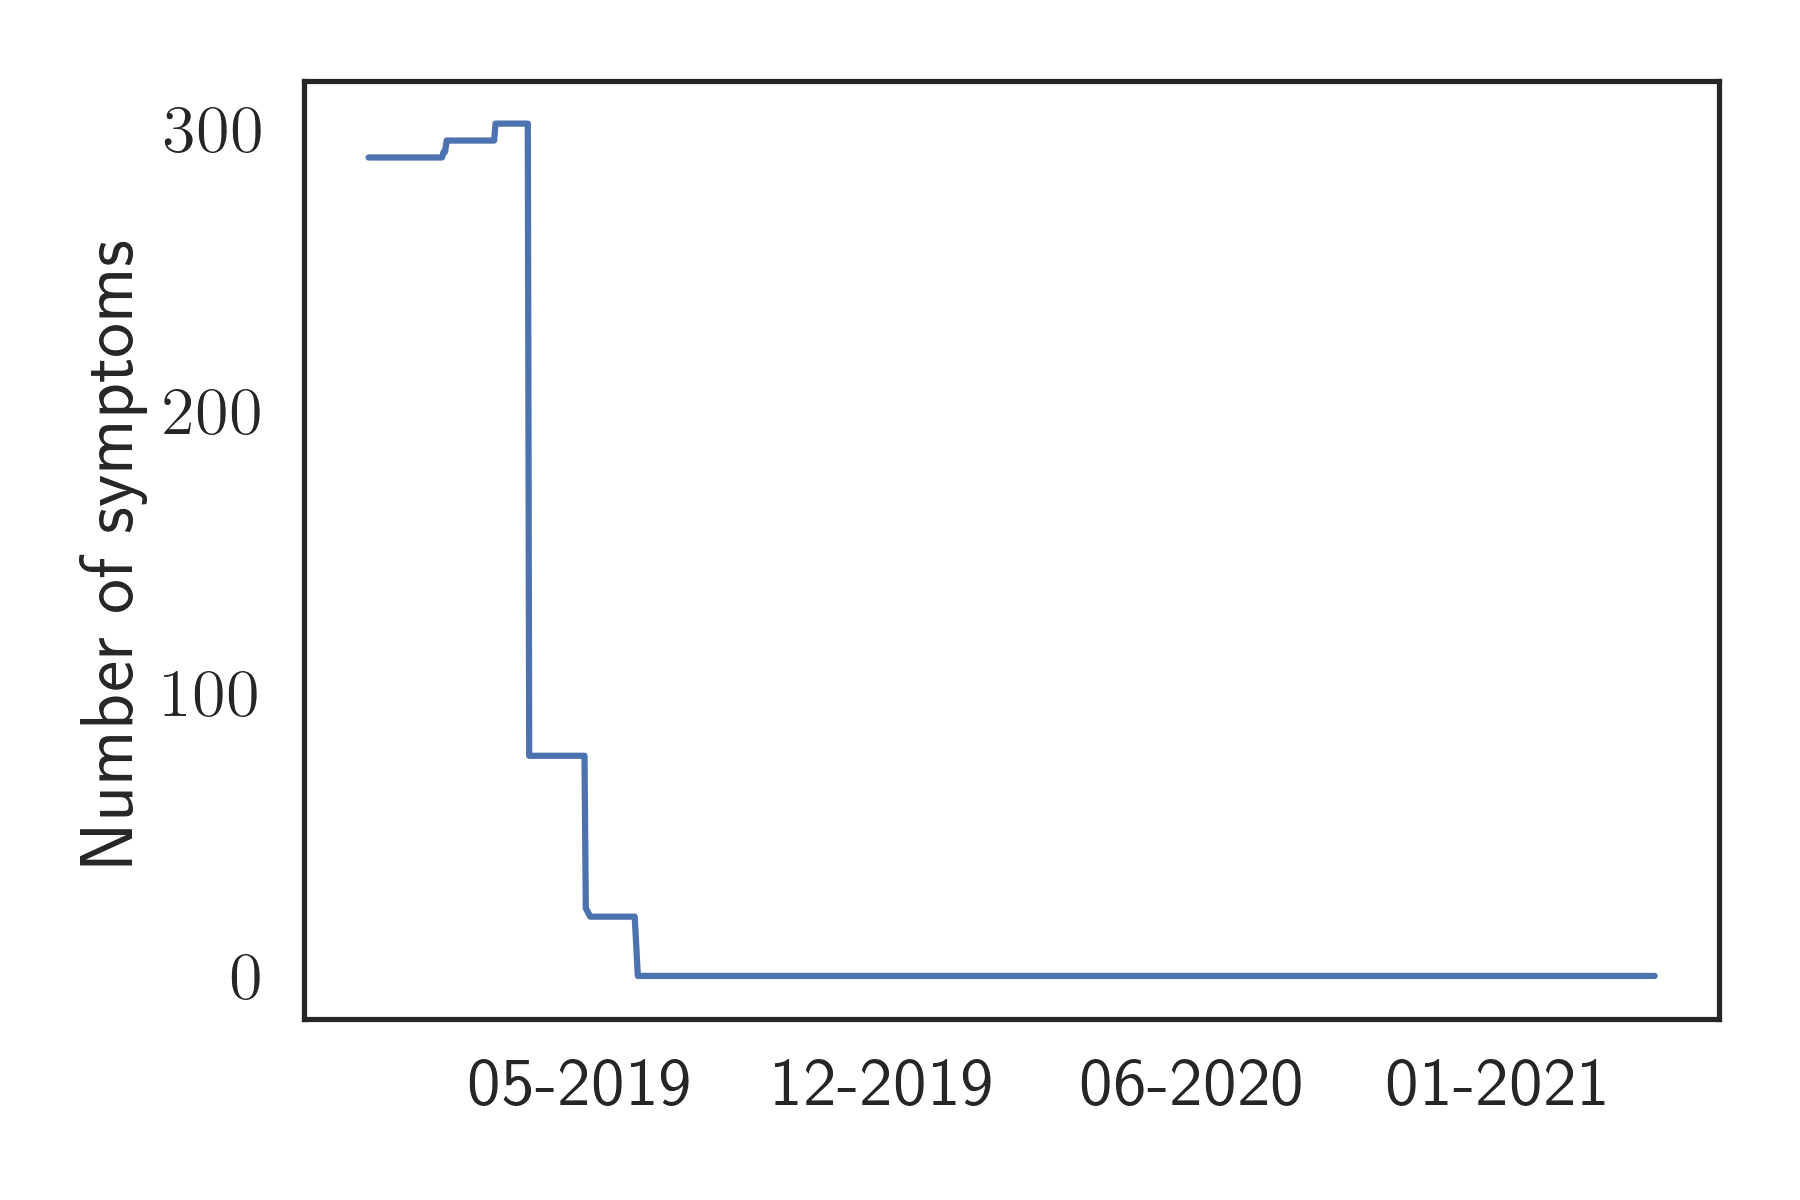
\includegraphics[width=0.5\linewidth]{figures/smells/smell-raw-evolution-bgl-narcissistic.png}
\caption{Evolution of the number of symptoms for the smell \emph{Narcissistic} over time for the industrial project (BGL BNP Paribas).}  
\label{fig:evolution-bgl-narcissistic}
\end{figure} 

The results for the open source projects depict a similar picture. Symptoms for \emph{Missing Assertion}, \emph{Middle Man}, \emph{Army of Clones}, and \emph{HardCoded Values} show also relatively high values compared to other symptoms. Similarly, we also notice a relatively large number of refactoring actions for the symptoms of \emph{Stinky Synchronization}, \emph{Over Checking}, and \emph{Lack of Encapsulation}. The difference between the results from \emph{Stinky Synchronization} can explain by the active policy in the industrial team preventing such symptoms to appear altogether.

Finally, similarly to Section~\ref{sec:results-smells-diffusion}, we perform a rank analysis using the normalized Levenshtein similarity. The value obtain when comparing the number of fixes performed in open-source and industrial projects is $0.4375$ and $0.2667$ when accounting for the percentage of refactoring. These low values show that the majority of the refactoring are not ranked in the same way in both industrial and open-source projects. Taking into account the results of Section~\ref{sec:results-smells-diffusion} this comparison suggest that when generalizing results obtained from open source projects, researchers should remain careful as their applicability in industrial context.

In conclusion, the results presented in this section show that the refactoring operation performed in industry and open-source projects present differences in term of which type of actions occurs the most often. However, in both cases, the proportion of symptomatic tests that are refactored remain low with the exception of the symptoms for \emph{Missing Assertion}. Indeed, for half of the categories less than 5\% of the symptomatic tests are ever subjects to refactoring. \emph{Missing assertion} is a unique exception with between 70\% (open-source) and 90\% (industrial) of the symptomatic tests being refactored. Interestingly, while refactoring actions are rare, test smells like \emph{Narcissistic} and \emph{Middle Man} still disappear from the test code base as a side effect of the replacement of symptomatic tests by new tests not exhibiting the symptom.